%%%%%%%%%%%%%%%%%%%%%%%%%%%%%%%%%%%%%%%%%
% Classic Lined Title Page 
% LaTeX Template
% Version 1.0 (27/12/12)
%
% This template has been downloaded from:
% http://www.LaTeXTemplates.com
%
% Original author:
% Peter Wilson (herries.press@earthlink.net)
%
% License:
% CC BY-NC-SA 3.0 (http://creativecommons.org/licenses/by-nc-sa/3.0/)
% 
% Instructions for using this template:
% This title page compiles as is. If you wish to include this title page in 
% another document, you will need to copy everything before 
% \begin{document} into the preamble of your document. The title page is
% then included using \titleAT within your document.
%
%%%%%%%%%%%%%%%%%%%%%%%%%%%%%%%%%%%%%%%%%

%----------------------------------------------------------------------------------------
%	PACKAGES AND OTHER DOCUMENT CONFIGURATIONS
%----------------------------------------------------------------------------------------



\documentclass[a4paper]{article}

\usepackage[utf8]{inputenc}
\usepackage{hyperref}
\usepackage{titlesec}
\usepackage{amssymb,amsmath}
\usepackage[italian]{babel}
\usepackage[titles]{tocloft}
\usepackage{appendix}
\hypersetup{%
    pdfborder = {0 0 0}
}
\usepackage{graphicx}
\usepackage{lastpage}
\usepackage{fancyhdr}
\usepackage{color}

\usepackage[svgnames]{xcolor} % Required to specify font color

\newcommand*{\plogo}{\fbox{$\mathcal{PL}$}} % Generic publisher logo

%----------------------------------------------------------------------------------------
%	TITLE PAGE
%----------------------------------------------------------------------------------------

\newcommand*{\titleAT}{\begingroup % Create the command for including the title page in the document
\newlength{\drop} % Command for generating a specific amount of whitespace
\drop=0.1\textheight % Define the command as 10% of the total text height

\rule{\textwidth}{1pt}\par % Thick horizontal line
\vspace{2pt}\vspace{-\baselineskip} % Whitespace between lines
\rule{\textwidth}{0.4pt}\par % Thin horizontal line

\vspace{\drop} % Whitespace between the top lines and title
\centering % Center all text
\textcolor{Black}{ % Red font color
{\Huge Appunti}\\[0.5\baselineskip] % Title line 1
{\Large di}\\[0.75\baselineskip] % Title line 2
{\Huge Reti e sicurezza}} % Title line 3

\vspace{0.25\drop} % Whitespace between the title and short horizontal line
\rule{0.3\textwidth}{0.4pt}\par % Short horizontal line under the title
\vspace{\drop} % Whitespace between the thin horizontal line and the author name

{\Large Luca De Franceschi\\Mirko Polato}\par % Author name

\vfill % Whitespace between the author name and publisher text
{\large Università degli studi di Padova}\par % Publisher

\vspace*{\drop} % Whitespace under the publisher text

\rule{\textwidth}{0.4pt}\par % Thin horizontal line
\vspace{2pt}\vspace{-\baselineskip} % Whitespace between lines
\rule{\textwidth}{1pt}\par % Thick horizontal line

\endgroup}

\titleformat{\chapter}[display]
{}{\hfill\rule{.7\textwidth}{3pt}}{2pt}
{\hspace*{.3\textwidth}\huge\bfseries}[\addvspace{1pt}]
\titleformat{name=\chapter,numberless}[display]
{}{\hfill\rule{.7\textwidth}{3pt}}{2pt}
{\hspace*{.3\textwidth}\huge\bfseries}[\addvspace{1pt}]

\renewcommand*\contentsname{Indice}

\newcommand{\glossario}[1]{\textit{#1\ped{G}}}

%----------------------------------------------------------------------------------------
%	BLANK DOCUMENT
%----------------------------------------------------------------------------------------

\begin{document}
\raggedright
\titleAT % This command includes the title page
\thispagestyle{empty}
\newpage

\pagenumbering{arabic}

\tableofcontents
\clearpage

\section{Introduzione}

La convergenza di computer e comunicazioni ha avuto un'influenza profonda sul modo in cui sono strutturati i calcolatori. Il concetto di ``centro di calcolo'' come una stanza con un grande computer dove gli utenti portano il loro lavoro per l'elaborazione oggi è completamente superato. Il vecchio modello di un solo computer che soddisfa l'intera necessità di calcolo dell'organizzazione è stato sostituito da un altro, in cui il lavoro è svolto da un gran numero di computer distinti ma interconnessi. Questi sistemi sono chiamati \textbf{reti di calcolatori}. Due computer sono interconnessi se sono in grado di scambiare informazioni tra di loro.

\subsection{Scopi delle reti di calcolatori}

L'obiettivo della \textbf{condivisione delle risorse} è quello di rendere disponibili a chiunque sulla rete tutti i programmi, le periferiche e soprattutto i dati, indipendentemente dalla posizione fisica dell'utente e della risorsa.
\linebreak
\linebreak
Nella sua forma più semplice, ci si può immaginare il sistema informatico di un'azienda come formato da uno o più database e da un certo numero di impiegati che hanno bisogno di accedervi remotamente. In questo modello i dati sono memorizzati in computer ad alte prestazioi chiamati \textbf{server}. Al contrario gli impiegati devono poter accedere ai dati e hanno sulla loro scrivania macchine più semplici chiamate \textbf{client}. Le macchine client e server sono collegate da una \textbf{rete}. Questa configurazione è chiamata \textbf{modello client-server}.

\begin{figure}[htbp]
\centering
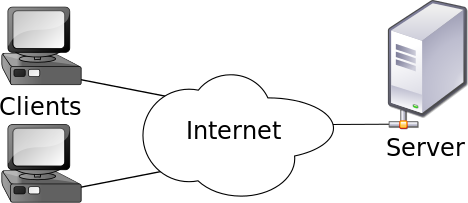
\includegraphics[width=50mm]{images/client-server-model.png}
\caption{Modello client-server}
\end{figure}

La comunicazione è rappresentata da un processo client che manda un messaggio attraverso la rete al processo server e resta in attesa di un messaggio di risposta. Quando il processo server riceve la richiesta esegue il lavoro o recupera i dati desiderati e manda indietro una risposta.

Una rete di calcolatori è un potentissimo \textbf{mezzo di comunicazione}. Alcuni esempi di utilizzo sono i seguenti:

\begin{itemize}

\item Comunicazione tramite \textbf{email};
\item Cooperazione tra gruppi distanti tra loro;
\item Videoconferenze;
\item Realizzare affari in modo elettronico;
\item Commercio elettronico (\textbf{e-commerce});
\item \textbf{Instant messaging};
\item Chat;
\item Comunicazione \textbf{peer-to-peer};
\item Insegnamento a distanza (e-learning);
\item Video on demand;

\end{itemize} 

\subsection{Hardware di rete}

Ci sono due tipi di tecnologie trasmissive impiegate a largo spettro:

\begin{enumerate}

\item Collegamenti broadcast (\textit{broadcast links});
\item Collegamenti punto-punto (\textit{point-to-point links}).

\end{enumerate}

Le \textbf{reti broadcast} hanno un solo canale di comunicazione che è condiviso fra tutte le macchine della rete. Brevi messaggi, chiamati in alcuni contesti \textbf{pacchetti}, sono inviati da ciascuna macchina e ricevuti da tutte le altre. Un campo indirizzo nel pacchetto individua il destinatario, l'indirizzo viene verificato e il pacchetto ricevuto.
\linebreak
\linebreak
Le \textbf{punto-punto}, al contrario, consistono di molte connessioni tra singole coppie di macchine, chiamate \textit{unicasting}. Per andare dalla sorgente alla destinazione, in questo tipo di rete un pacchetto deve visitare una o più macchine intermedie.
\linebreak
\linebreak
Un criterio alternativo per classificare le reti è la loro \textbf{scala}:

\begin{figure}[htbp]
\centering
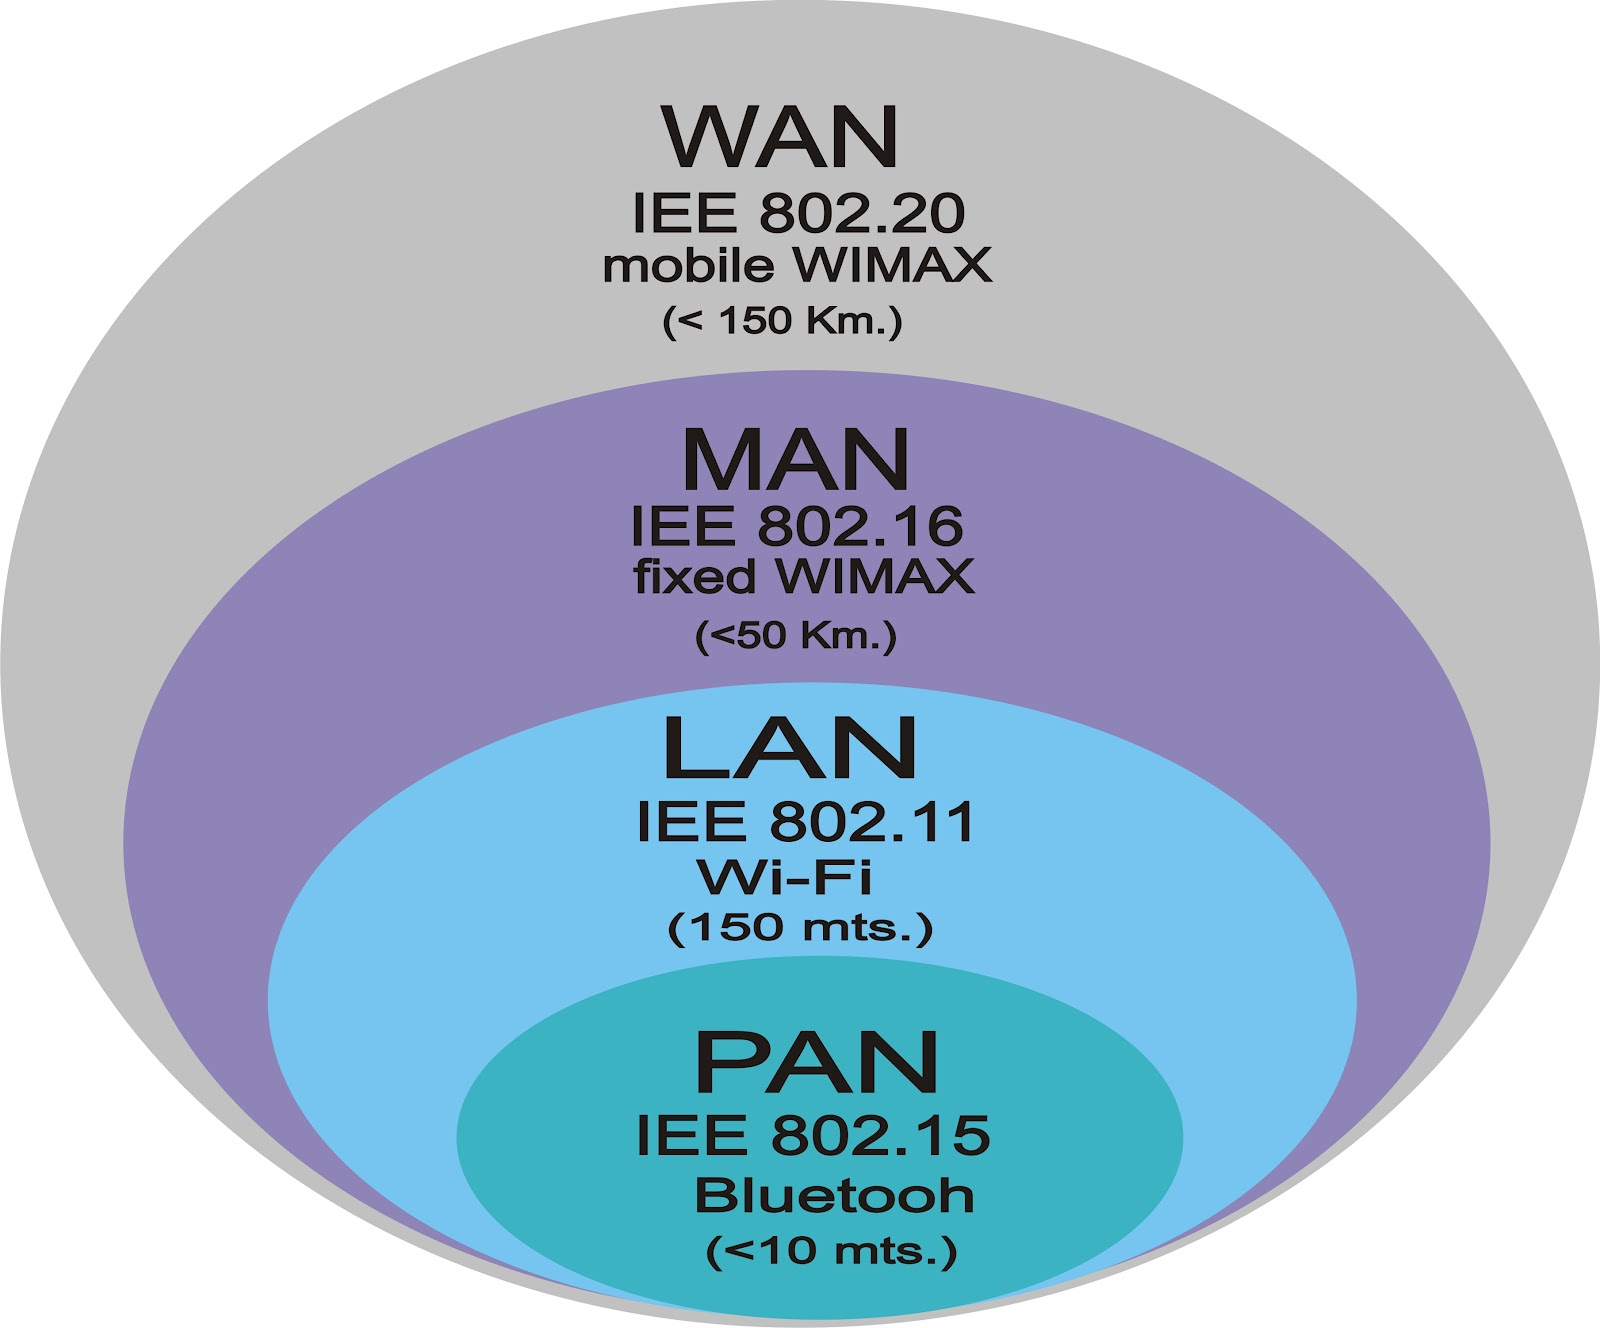
\includegraphics[width=50mm]{images/scala-reti.jpg}
\caption{Classificazione delle reti in base alla scala}
\end{figure}

Le reti locali, solitamente chiamate LAN, sono reti private installate all'interno di un singolo edificio, con dimensione fino a qualche Km, hanno dimensioni contenute e lavorano normalmente a velocità comprese tra 10 Mbps e 100 Mbps. Dispongono di due diverse topologie di trasmissione:

\begin{enumerate}

\item Rete a bus, in cui in ogni istante si può trasmettere a una macchina;
\item Rete ad anello, in cui ogni bit si propaga in modo autonomo senza aspettare il resto del pacchetto;

\end{enumerate}

\begin{figure}[htbp]
\centering
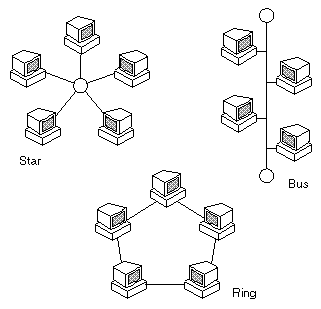
\includegraphics[width=50mm]{images/lan-topologia.png}
\caption{Diverse topologie delle reti LAN}
\end{figure}

Una rete metropolitana (\textit{Metropolitan Area Network}) copre un'intera città. L'esempio più noto di MAN è la rete di televisione via cavo disponibile in molte città degli Stati Uniti. La distribuzione delle informazioni nelle abitazioni avviene tramite una stazione di testa centralizzata.
\linebreak
\linebreak
Una \textit{Wide Area Network} o WAN copre un'area geograficamente estesa, spesso una nazione o un continente. Racchiude una serie di macchine destinate a eseguire programmi utente, chiamate \textbf{host}. Gli host sono collegati da una \textbf{communication subnet}, che trasporta i messaggi da un host all'altro ed è generalmente gestita da una compagnia telefonica o da un Internet provider. Le \textbf{linee di trasmissione} spostano i bit tra le macchine. Gli \textbf{elementi di commutazione} sono computer specializzati che collegano tre o più linee di trasmissione. Quando i dati arrivano da una linea ricevente, l'elemento di commutazione deve scegliere una linea di uscita su cui inoltrarlo. Questo viene eseguito dal \textbf{router}. Il modo in cui un router decide come mandare il messaggio si chiama \textbf{algoritmo di routing}.

\begin{figure}[htbp]
\centering
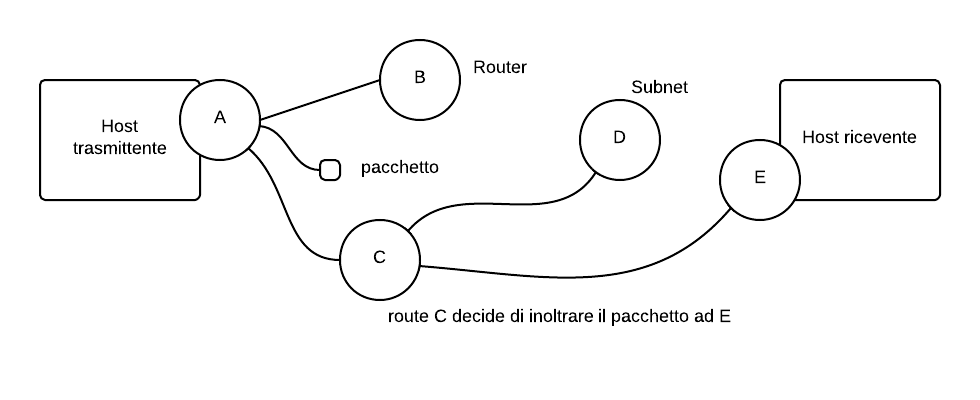
\includegraphics[width=100mm]{images/wan.png}
\caption{Schema di una rete WAN}
\end{figure}

\subsection{Software di rete}

Per diminuire la complessità, la maggior parte delle reti è organizzata come pila di \textbf{strati} (\textit{layer}) o \textbf{livelli}, costruiti uno sull'altro. Lo scopo di ogni strato è quello di offrire determinati servizi agli strati di livello superiore, schermandoli dai dettagli sull'implementazione dei servizi (\textit{information hiding}).
Lo strato \textit{n} di un computer è in comunicazione con lo strato \textit{n} di un altro computer e la comunicazione è regolamentata da \textbf{protocolli}. Fondamentalmente un protocollo è un accordo, tra le parti che comunicano, sul modo in cui deve procedere la comunicazione (formato, ordine in cui i messaggi vengono inviati e ricevuti, azioni da prendere, ...). 
Tra ogni strato contiguo esiste inoltre un'\textbf{interfaccia}, che definisce le operazioni elementari e i servizi che lo strato inferiore rende disponibili a quello soprastante.

\begin{figure}[htbp]
\centering
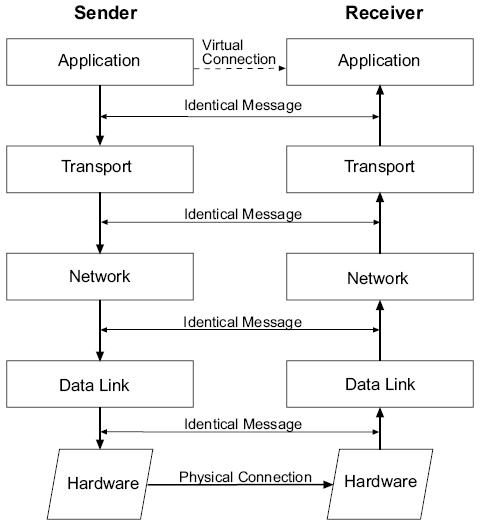
\includegraphics[width=80mm]{images/layers.jpg}
\caption{Organizzazione a strati}
\end{figure}

L'insieme di strati e di protocolli si chiama \textbf{altrorchitettura di rete} (non ne fanno parte le interfacce perchè nascoste dal computer). Un elenco di protocolli usati da uno specifico computer si chiama \textbf{pila di protocolli}.
\linebreak
\linebreak
Gli strati possono offrire due tipi di servizio a quelli sovrastati: orientati alla connessione oppure senza connessione. Un servizio \textbf{orientato alla connessione} assomiglia al sistema telefonico: il trasmettitore spinge gli oggetti (bit) da un estremità (come un tubo) e il ricevitore li prende dall'altra. In alcuni casi il ricevitore e la subnet eseguono una \textbf{negoziazione} dei parametri da usare. 
Al contrario, un servizio \textbf{senza connessione} si comporta come la posta: ogni messaggio trasporta l'indirizzo completo del destinatario ed è instradato attraverso il sistema postale in modo indipendente dagli altri.

\subsection{Il modello di riferimento OSI}

Il modello OSI (\textit{Open System Interconnection}) ha sette strati. I principi che sono stati applicati per arrivare ai sette strati si possono brevemente riassumere come segue:

\begin{enumerate}

\item Si deve creare uno strato quando è richiesta un'astrazione diversa;
\item Ogni strato deve svolgere una funzione ben definita;
\item La funzione di ogni strato va scelta con uno sguardo rivolto alla definizione di protocolli internazionali;
\item I confini degli strati vanno scelti per minimizzare il flusso d'infomrazioni attraverso le interfacce;
\item Il numero di strati deve bastare per evitare la necessità di radunare funzioni distinte nello stesso strato, ma essere abbastanza piccolo da rendere l'architettura instabile.

\end{enumerate}

Lo \textbf{strato fisico} si occupa della trasmissione di bit grezzi sul canale di comunicazione. I requisiti di progetto devono assicurare che ogni bit trasmesso con valore 1 sia ricevuto ancora come 1, e non come 0.
\linebreak
\linebreak
Il compito dello \textbf{strato data link} consiste nel cercare di rilevare, per quanto possibile, gli errori di trasmissione così da evitare di trasmettere questi errori riconosciuti al livello superiore.
\linebreak
\linebreak
Lo \textbf{strato network} controlla il funzionamento della subnet. Un problema chiave riguarda la modalità con cui i pacchetti sono inoltrati dalla sorgente alla destinazione.
\linebreak
\linebreak
La funzione essenziale dello \textbf{strato trasporto} è quella di accettare dati dallo strato superiore, dividerli in unità più piccole quando necessario, passarle allo strato network e assicurarsi che tutti i pezzi arrivino correttamente all'altra estremità.
\linebreak
\linebreak
Lo \textbf{strato applicazione} comprende una varietà di protocolli comunemente richiesti dagli utenti. Un protocollo applicativo largamente utilizzato è HTTP.
\clearpage
\section{Lo strato fisico}

Lo scopo dello strato fisico è quello di trasportare un flusso di bit da una macchina all'altra. I mezzi di trasmissione si dividono in:

\begin{itemize}

\item Mezzi di trasmissione \textbf{guidati};
\item Mezzi di trasmissione \textbf{non guidati}.

\end{itemize}

\subsection{Basi teoriche della comunicazione dati}

Le informazioni posso essere trasmesse via cavo variando alcue proprietà fisiche (tensione/corrente). Rappresentando la tensione/corrente in una funzione f(t) è possibile analizzare il segnale. Fourier dimostrò che un segnale di questo tipo, periodico e abbastanza regolare può essere descritto da una ideale somma infinita di seni e coseni:

$$g(t)=\frac{1}{2}c+\displaystyle\sum\limits_{n=1}^\infty a_n sen(2\pi nft)+\displaystyle\sum\limits_{n=1}^\infty b_n cos(2\pi nft) $$

dove $f=1/T$ rappresenta la frequenza fondamentale, $a_n$ e $b_n$ sono rispettivamente le ampiezze seno e coseno della \textit{n-esima} \textbf{armonica}, e $c$ rappresenta una costante. Questa scomposizione è chiamata \textbf{serie di Fourier}.
\linebreak
\linebreak
L'intervallo di frequenze trasmesse senza una forte attenuazione è chiamato \textbf{banda passante}, o semplicemente banda, ovvero l'insieme di frequenze che riescono a trasmettere sul canale, misurata in \textit{Hertz}. La banda passante è una proprietà fisica del mezzo di trasmissione e di solito dipende dalla \textit{costruzione}, dallo \textit{spessore} e dalla \textit{lunghezza} del mezzo. Nessun mezzo trasmissivo è perfetto, per cui c'è sicuramente attenuazione del segnale. Anche in un canale perfetto ci si accorge comunque che un segnale digitale non può essere trasmesso a velocità troppo elevate, esistono però alcuni schemi di codifica per aumentare la velocità di trasmissione.

Una funzione può essere ricostruita  a partire dalla sua serie di Fourier. Analizziamo un segnale di trasmissione analogica e proviamo a ricostruirlo con Fourier. Dobbiamo tener conto che nessun canale trasmissivo è perfetto, per cui c'è sicuramente attenuazione. L'intervallo di frequenze trasmesse senza forte attenuazione è detto \textbf{banda passante}. Anche in un canale perfetto ci si accorge comunque che un segnale digitale non può essere trasmesso a velocità troppo elevate, esistono però alcuni schemi di codifica per aumentare la velocità di trasmissione.\\
Henry Nyquist (ingegnere di AT\&T) e Claude Shannon dimostrarono che la velocità massima di trasmissione è:\\

\[V_{max} = 2H\log_{2}V bit/sec\]

Mentre il livello di rumore si misura facendo il \textbf{rapporto segnale-rumore}. Solitamente viene indicata tale misura antecedendo \(10log_{10}\) e misurando in dB.

\[Segnale/Rumore = 10log_{10} S/N dB\]

Un risultato notevole ottenuto da Shannon fu:

\[MAX_{bit/s} = H log_{2}(1 + S/N)\]

con H pari all'ampiezza di banda in Hz.

\subsection{Mezzi di trasmissione guidati}

\subsubsection{Mezzi Magnetici}

Sistema molto semplice, utilizzato da sempre e basato su un funzionamento banale: si salvano i dati su nastri magnetici (dischi rimovibili) e si trasportano fisicamente a destinazione dove verranno letti. Se si pensa a un tir che trasporta un centinaio di HD da 1TB che percorre qualche Km per consegnare questi dischi si può intuire che la larghezza di banda è elevatissima e con un costo irrisorio. La cosa banalmente poco buona è l'enorme ritardo nella trasmissione dati, in quanto la durata della trasmissione è espressa in minuti e in ore, non in millisecondi.

\subsubsection{Doppino}

È uno dei mezzi di trasmissione più vecchi, ma è ancora molto in voga. Il doppino è composto da 2 conduttori di rame isolati (spessi 1mm), attorcigliati tra loro a forma elicoidale (stile DNA), questo per evitare interferenze tra di loro (risulterebbero un ottima antenna), in quanto i campi elettromagnetici generati dai due conduttori si annullano a vicenda. Viene largamente utilizzato nel sistema telefonico, questo perché il doppino può attraversare diversi Km senza bisogno di amplificare il segnale così dall'abitazione si può agevolmente arrivare alla centrale. Si possono usare per trasmettere dati Analogici o anche Digitali e la larghezza di banda dipende dal diametro del cavo e dalla distanza percorsa. Esistono più categorie di questi cavi che differiscono sostanzialmente per il numero di spire per cm per ridurre le interferenze. Il doppino \textbf{cat3} (usato sino al 1988) è composto da 2 cavi isolati e attorcigliati. Il doppino \textbf{cat5} è come il cat3, ma utilizza più spire per cm; questo lo rende più adatto a trasmissione ad alta velocità in quanto migliora la qualità del segnale. Il doppino può arrivare a una banda di 250-600MHz. Questi cavi sono detti anche UTP (\textit{Unshielded Twisted Pair}).

\subsubsection{Cavo coassiale}
	
Essendo più schermato del precedente il \textbf{cavo coassiale} può estendersi per distanze maggiori. Esistono 2 tipi di cavi coassiali: da 50 Ohm per le trasmissioni digitali e da 75 Ohm per le analogiche, per la televisione e le connessioni Internet via cavo. 
È composto da un nucleo di rame, rivestito da materiale isolante a sua volta rivestito da una calza conduttrice il tutto ricoperto da una guaina protettiva, il cavo coassiale è caratterizzato da un eccellente immunità al rumore. L'ampiezza di banda di questi cavi arriva attorno a 1GHz e dipende dalla lunghezza, dalla qualità e dal rapporto segnale-rumore del segnale. Il cavo coassiale è ancora molto utilizzato per le reti metropolitane e le televisioni via cavo.

\begin{figure}[htbp]
\centering

\includegraphics[width=80mm]{images/cavo_coassiale.jpg}
\caption{Struttura del cavo coassiale}
\end{figure}

\subsubsection{Fibra Ottica}

Un sistema di trasmissione ottico è formato principalmente di 3 parti: \textbf{sorgente luminosa}, \textbf{mezzo di trasmissione} e \textbf{rilevatore di luce}. Per convenzione, un impulso di luce indica il valore 1 e l'assenza di luce indica il valore 0. Il mezzo trasmissivo ovviamente è la fibra composta da un nucleo (\textbf{core}) di vetro di pochi micron avvolto in una guaina di vetro (\textbf{cladding}) con indice di rifrazione più basso e infine la solita rivestitura con guaina in plastica. La fibra si basa su un principio molto semplice, ovvero che la luce che la attraversa viene riflessa al suo interno fino ad arrivare all'altra estremità del cavo. Questo avviene perchè la luce immessa nel core incontra il cladding con indice di rifrazione minore e il raggio luminoso viene così riflesso (se possiede un inclinazione corretta). La velocità di tale raggio è circa quella della luce, infatti il limite di banda della fibra non è dovuto alla velocità di trasmissione ma di decodifica del segnale luminoso in impulso elettrico. Una fibra può contenere più raggi che si riflettono in essa l'importante è che il loro angolo di riflessione sia diverso. Questo tipo di fibre è detto \textbf{multimodale}. Le fibre che invece permettono la trasmissione di luce in linea retta sono le \textbf{monomodali} che non sono altro che guide d'onda ma possono raggiungere i 50Gbps per 100Km senza attenuazione.

L'attenuazione della luce attraverso il vetro dipende dalla lunghezza d'onda della luce. L'attenuazione, espressa in decibel, si ricava dalla seguente formula:

$$attenuazione = 10\log_{10} \frac{energia trasmessa}{energia ricevuta} $$

Per la comunicazione ottica si usano tre bande di lunghezza d'onda, centrate rispettivamente a 0,85, 1,30 e 1,55 micron. Gli impulsi luminosi trasmessi attraverso la fibra si espandono in lunghezza durante la propagazione; il fenomeno si chiama \textbf{dispersione cromatica}, che dipende dalla lunghezza d'onda. 
\linebreak
\linebreak
Per generare il segnale normalmente si impiegano due tipi di sorgenti luminose: i \textbf{LED} (\textit{Light Emitting Diode}) e i \textbf{semiconduttori laser}. All'estremità finale della fibra si trova un fotodiodo che genera un impulso elettrico ogni volta che è colpito dalla luce. Il tipico tempo di risposta di un fotodiodo è un nsec, perciò la trasmissione dati è limitata a 1 Gpbs.
\linebreak
\linebreak
Un problema delle fibre è il collegamento tra 2 di esse, che può avvenire in 3 modi:

\begin{enumerate}

\item{Le fibre vengono inserite in apposite prese grazie a dei connettori con perdita di circa 10-20\% della luce};
\item{Le fibre vengono attaccate meccanicamente, messe di fronte una all'altra e poi viene avvolto in una macchina particolare per poi essere pinzate, con perdita comunque di circa il 10\% della luce};
\item{Le fibre vengono fuse tra loro. Una soluzione quasi ottimale, anche se difficile, genera una piccola attenuazione di segnale}.

\end{enumerate}

Le LAN basate sulle fibre ottiche solitamente sono ad anello con congiunzione a T per ogni pc o a stella passiva, questo per evitare gli ostacoli. La configurazione ad anello ha il difetto che se una congiunzione si guasta salta tutta la rete. Altre topologie di configurazione possono essere quelle a \textbf{stella passiva}
\linebreak
\linebreak
Tra gli innumerevoli vantaggi della fibra ottica rispetto alle connessioni in rame citiamo:

\begin{itemize}

\item Maggiore ampiezza di banda;
\item Non viene influenzata dalle sorgenti elettriche;
\item Non viene influenzata dai campi magnetici e interruzioni della linea elettrica;
\item Sono molto più leggere;
\item Non perdono la luce;
\item L'intercettazione dei dati è molto difficile, quindi c'è una maggior sicurezza;

\end{itemize}

Di contro è una tecnologie ancora nuova e poco sviluppata e presenta grossi costi di manutenzione.

\subsubsection*{Tabella riassuntiva}

\begin{figure}[htpb]
\centering
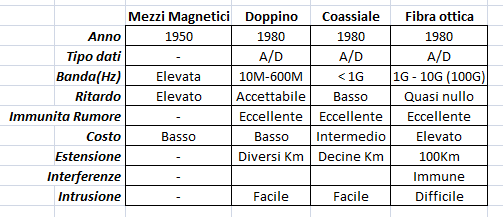
\includegraphics[scale=1]{images/mezzi.png}
\caption{Riassunto caratteristiche dei mezzi trasmissivi guidati}
\end{figure}	

\newpage

\subsection{Trasmissioni wireless}

\subsubsection{Lo spettro elettromagnetico}

Quando si spostano, gli elettroni creano onde elettromagnetiche che si propagano attraverso lo spazio, anche nel vuoto. Questa osservazione fu fatta per la prima volta dal fisico tedesco Heirich Hertz. Il numero di oscillazioni al secondo di un'onda è chiamato \textbf{frequenza} e si misura in Hz. La distanza massima tra 2 picchi (o minimi) è chiamata \textbf{lunghezza d'onda} ed è universalmente indicata dalla lettera greca $\lambda$ (lambda).
Nel vuoto tutte le onde elettromagnetiche viaggiano alla stessa velocità, qualunque sia la loro frequenza. Questa velocità, chiamta \textbf{velocità della luce} \textit{c}, è pari a circa $3*10^8 m/sec$. Nei cavi in rame e nelle fibre ottiche la velocità di trasmissione scende a 2/3. La velocità della luce è il limite ultimo della velocità: nessun oggetto o segnale può muoversi più velocemente.
La relazione fondamentale tra $f$, $\lambda$ e \textit{c} (nel vuoto) è:

$$\lambda f = c$$

Tutte le trasmissioni wireless si basano sul principio che un antenna collegata a un circuito elettrico invia onde elettromagnetiche che possono essere captate da un ricevitore posto a una distanza appropriata. Qui di seguito è visualizzato lo spettro elettromagnetico e la sua suddivisione.

\begin{figure}[htpb]
\centering
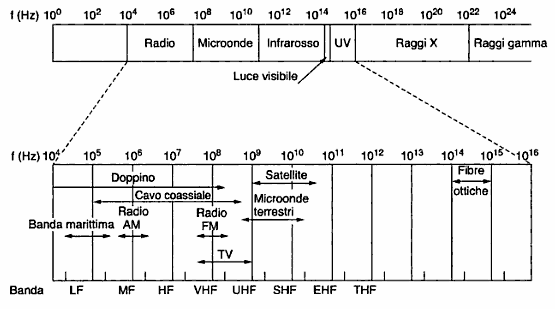
\includegraphics[scale=1]{images/spettro.png}
\caption{Spettro elettromagnetico.}
\end{figure}

La quantità di informazione che un'onda elettromagnetica può trasportare dipende dalla sua banda. La maggior parte delle trasmissioni utilizza una banda di frequenza ristretta per ottenere la migliore ricezione, ma in certi casi si usa una banda larga con due varianti. Nella tecnica a \textbf{spettro distribuito a frequenza variabile}, il trasmettitore salta da una frequenza a un'altra centinaia di volte al secondo. Questa variante è utilizzata nelle comunicazioni militari, perchè rende difficile rilevare le trasmissioni ed è quasi impossibile da disturbare.
L'altra forma di trasmissione, chiamata \textbf{spettro distribuito a frequenza diretta}, propaga il segnale in banda larga ed è stato utilizzato per alcuni modelli di cellulari di seconda generazione.

\subsubsection{Trasmissioni radio}

Le onde radio sono onde omnidirezionali semplici da riprodurre e viaggiano per lunghe distanze attraversando gli edifici. Non necessita di alcun allineamento trasmettitore-ricevente. Le proprietà delle onde radio dipendono dalla loro frequenza. Nell'aria l'attenuazione delle onde con frequenze più basse è di circa 1/\(r^2\). Nelle bande VLF, LF, MF le onde seguono la forma del terreno e la curvatura della terra e possono viaggiare per circa 1000 Km. Alle frequenze più alte (HF) invece le onde tendono a viaggiare in linea retta, rimbalzando sugli ostacoli (ionosfera) e sono assorbite dalla pioggia. 
A tutte le frequenze le onde radio sono soggette a interferenze da parte di motori e altri dispositivi elettrici. 

\subsubsection{Trasmissione a microonde}

Sopra i 100 MHz le onde viaggiano quasi in linea retta per cui è necessario un allineamento trasmettitore-ricevente. Concentrando l'onda in un piccolo raggio si ottiene un ottimo rapporto segnale/rumore. Il problema di queste trasmissioni sta nelle lunghe distanze e dalla curvatura della terra, la quale porta alla necessità di ripetitori. L'utilizzo di antenne molto alte riduce l'effetto della curvatura. Più sono le antenne, maggiore può essere la loro distanza. La distanza tra ripetitori varia grossolanamente con la radice quadrata dell'altezza dell'antenna. 
Alcune onde posso rinfrangersi negli strati più bassi dell'atmosfera e arrivare in ritardo rispetto a quelle dirette e addirittura fuori fase causandone l'annullamento (\textbf{multipath fading}). Le microonde non attraversano gli edifici molto bene, e sono soggette alle condizioni climatiche. Comunemente si usano bande sopra i 10 GHZ ma sopra i 40 GHz la pioggia comincia ad assorbire le onde. Questo sistema di trasmissione offre diversi vantaggi rispetto alla fibra; il principale è che non richiede alcun diritto di passaggio: acquistando un piccolo appezzamento di terreno ogni 50 Km e costruendo su di esso un'antenna è possibile scavalcare il sistema telefonico e comunicare direttamente. Le microonde sono anche relativamente convenienti: acquisto e installazione di apparecchi per questo tipo di trasmissione è molto basso.

\subsubsection*{Divisione dello spettro elettromagnetico}

Tutti vogliono un pezzo di spettro per aumentare la velocità di trasmissione e quindi bisogna regolarne tale divisione, se ne occupa l'\textbf{ITU-T}. In passato per compiere tale divisione sono stati utilizzati 3 modi (3 algoritmi):

\begin{enumerate}

\item{\textbf{Concorso di bellezza}: ognuno di coloro che voleva spettro doveva dare un motivo per il quale doveva averlo proprio lui. Problemi: corruzioni e scelte arbitrarie senza senso;}
\item{\textbf{Lotteria}: veniva fatta una vera e propria lotteria per assegnare lo spettro. Problemi: partecipavano anche i non interessanti solo per guadagnare soldi dalla rivendita dello spettro;}
\item{\textbf{Asta}: vendita all'asta dello spettro. Problema: banca rotta delle aziende a causa dei debiti.}

\end{enumerate}

Un approccio completamente differente consiste nel non assegnare affatto le frequenze, lasciando che ognuno trasmetta a piacere, ma regolando la potenza utilizzata in modo da limitare la portata delle stazioni per evitare l'interferenza reciproca. Seguendo questo principio la maggior parte dei governi ha riservato alcune bande di frequenza, chiamate \textbf{ISM} (\textit{Industrial}, \textit{Scientific}, \textit{Medical}), per l'utilizzo senza licenze.

\subsubsection{Infrarossi}

Sistema economico e facile da costruire con il difetto di non riuscire ad attraversare gli ostacoli. Queste onde, infatti, si avvicinano alle onde di tipo luminose. Sono più sicuri delle onde radio per la difficoltà di intercettazione, ma risentono molto degli ostacoli. Questo a volte può rappresentare anche un vantaggio (es. telecomandi tv). Per questi motivi sono usati per distanze brevi (collegamento pc-stampanti, telecomandi ecc..), e hanno un ruolo secondario nelle telecomunicazioni. Il sistema infrarosso non richiede alcuna licenza governativa.

\subsubsection{Trasmissioni a onde luminose (LASER)}

Sistema poco costoso che offre una banda molto elevata, facile da installare e non richiede licenze. La sua debolezza sta nel raggio molto sottile (e unidirezioneale) e quindi difficile da indirizzare verso il bersaglio esatto. Per ovviare al problema a volte vengono inserite lenti per rendere il raggio meno focalizzato. Il raggio laser per di più non attraversa la pioggia e la nebbia ed è soggetto a fenomeni di convezione (turbolenza provocata da fonti di calore).

\subsection{Comunicazioni satellitari}

Nella sua forma più semplice un satellite può essere immaginato come un grande ripetitore di microonde collocato nel cielo, che contiene molti \textbf{trasponder} (ricetrasmettitori satellitari). Ciascuno di questi ascolta una parte dello spettro, amplifica il segnale in ingresso e lo ritrasmette su un'altra frequenza per evitare interferenze con il segnale in arrivo. I raggi puntati verso la terra possono essere larghi oppure stretti, questa modalità operativa è detta \textbf{bent pipe}. I satelliti hanno un periodo orbitale che dipende dalla loro altezza rispetto alla terra. Più è alto un satellite, più è lungo il suo periodo. Un problema è la presenza delle \textbf{fasce di Val Allen}, strati di particelle molto cariche, che distruggerebbero in poco tempo un satellite che le attraversasse.

\begin{figure}[htpb]
\centering
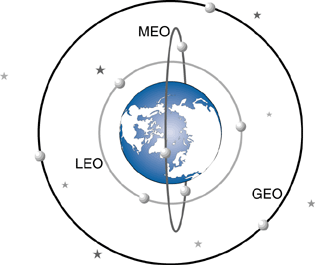
\includegraphics[scale=1]{images/Orbits.png}
\caption{Posizione dei salettiti GEO, MEO e LEO}
\end{figure}

\subsubsection{Satelliti Geostazionari (GEO)}	

Questi satelliti sono posti in orbite molto alte e con le tecnologie odierne non si possono collocare 2 satelliti GEO a meno di 2 gradi nel piano equatoriale, per evitare interferenze, quindi con $360/2=180$ satelliti si copre tutto. L'allocazione degli slot spaziali è gestito dall'\textbf{ITU}. L'ITU inoltre ha assegnato alcune bande di frequenza alle applicazioni satellitari in modo da non interferire con i sistemi a microonde preesistenti. 
I moderni satelliti possono raggiungere dimensioni enormi: alcuni pesano 4000 Kg e consumano diversi kilowatt di energia elettrica prodotta da pannelli solari. Gravità solare, lunare e planetaria tendono ad allontanarli dagli slot e dagli orientamenti assegnati, ma l'effetto è contrastato dai motori a razzo installati a bordo. La continua attività di messa punto è chiamata \textbf{station keeping} e quando dopo una decina di anni circa il propellente dei motori si esaurisce, il satellite va alla deriva e precipita senza che si possa far nulla, quindi dev'essere disattivato. 
\linebreak
\linebreak
I segnali inviata da questi satelliti viaggia alla velocità della luce, ma essendo molto lontani dalla terra hanno comunque un ritardo di circa 300 ms. I primi satelliti GEO con una singola emissione coprivano circa 1/3 della terra, chiamata \textbf{impronta}. Poi con lo sviluppo delle tecnologie si è cominciato a concentrare i raggi trasmissivi (spot) in aree geografiche più piccole (centinaia di Km). Un nuovo passo avanti nel settore delle comunicazioni satellitari si ebbe con le stazioni \textbf{VSAT}, piccole stazioni con un'antenna da circa 1m che comunicano con i satelliti GEO. Per le loro piccole dimensioni e potenza, non essendo in grado di comunicare tra loro, si è dovuto ideare alcune stazioni particolari più potenti per fare da ponte. Sono ovviamente mezzi di trasmissione broadcast e per quanto riguarda la sicurezza sono un disastro. Il costo della trasmissione satellitare non dipende dalla distanza, ma è costante. Hanno una reattività quasi istantanea e un ottimo tasso di errore.

\subsubsection{Satelliti su orbite medie (MEO)}

Questi satelliti sono disposti ad altitudini molto più basse, comprese tra le due fasce di Van Allen. Essi si muovono sopra di noi a una velocità relativamente bassa,percorrendo il giro del pianeta in circa 6 ore. Di conseguenza devono essere rintracciati mentre si spostano nel cielo. Coprono un'area più piccola dei GEO e si possono raggiungere con mezzi meno potenti. I 24 satelliti GPS che orbitano a 18000 Km sono di tipo MEO.

\subsubsection{Satelliti su orbite basse (LEO)}

Si spostano molto velocemente e per realizzare un sistema completo sono necessari molti satelliti di questo tipo. Essendo vicini alla crosta terrestre le stazioni non hanno bisogno di molta energia per comunicare con poco ritardo.

\subsubsection*{Iridium}					

Lanciati nel 1997 i 66 satelliti LEO del progetto \textbf{Iridium} (Motorola) vennero acquistati da un investitore riprendendo il servizio nel marzo 2001, che era stato fermato nel 1999. Il progetto fornisce un servizio di telecomunicazione a livello mondiale basato su ``cellulari particolari''. I satelliti Iridium sono collocati a 750 Km di altezza, con un satellite ogni 32 gradi. Le trasmissioni avvengono nello spazio: ogni satellite comunica con altri satelliti fino a destinazione.

\subsubsection*{GlobalStar}

Basato su 48 satelliti LEO utilizzando uno schema di commutazione diverso dal precedente. Il satellite che riceve la chiamata trasmette a una centrale terrestre che comunica con altre fino al satellite posto sulla cella del destinatario. La complessità resta quindi terrestre facilitandone la gestione.

\subsubsection*{Teledesic}

Progetto mirato per gli utenti internet, con l'idea di offrire 100 Mbps in trasmissione e 720 in ricezione. Il sistema è composto da 32 satelliti LEO con un impronta più grande. Basato sulla commutazione di pacchetto, con ogni satellite in grado di instradare ogni singolo pacchetto.

\subsubsection{Satelliti o fibra?}

E' ovvio che la comunicazione con le fibre sia molto veloce, ma ci sono molti settori in cui i satelliti non possono essere rimpiazzati dalla fibra, come ad esempio la comunicazione mobile. Le comunicazioni broadcast per eccellenza sono satellitari. Un altro settore è la comunicazione in luoghi ostili, in cui le infrastrutture terrestri scarseggiano e la posa di cavi ottici non sarebbe il massimo. Inoltre anche le zone in cui i costi di posa sono elevati il satellite può essere un ottima alternativa. In sostanza per la comunicazione terrestre è sicuramente migliore la fibra ma i satelliti rimarranno indispensabili per altri settori. Il futuro delle comunicazioni sembrerebbe essere comunque quello terrestre basato su fibre ottiche combinato con la rete cellulare, ma per alcune applicazioni specializzate i satelliti sono migliori.

\subsection{Sistema Telefonico}

\subsubsection{Struttura della rete}

Inizialmente il mercato dei telefoni prevedeva la vendita di 2 apparecchi e spettava all'utente tirare il cavo tra i 2 telefoni. Questo intuitivamente creò una struttura di rete troppo confusa. Bell notato questo particolare aprì il primo ufficio di commutazione nel 1878. Le chiamate quindi dovevano passare per la centrale nella quale un addetto si occupava di collegare con un cavo il chiamante al chiamato. La rete però, sebbene meno complessa, rimase ancora troppo confusa poichè non era pensabile collegare ogni ufficio di commutazione a una centrale. Vengono così ideati i livelli delle centrali di commutazione. Inizialmente con 2 livelli fino ad arrivare a 5. In generale una comunicazione avviene a più livelli:

\begin{enumerate}

\item{La richiesta di chiamata arriva alla centrale locale del chiamante alla quale è collegato direttamente con 2 cavi di rame (doppino di categoria 3). Se il chiamato appartiene alla stessa centrale locale avviene il collegamento tra le parti};
\item{La centrale locale è collegata a una centrale interurbana (con cavi in fibra/microonde/coassiale),e come per quella locale se la centrale locale del chiamato è collegata alla stessa centrale interurbana allora le parti si collegano};
\item{Le centrali interurbane sono connesse a centrali intermedie e la trasmissione avviene analogamente alle precedenti}.

\end{enumerate}

Le trasmissioni sono preferibili in digitale per la non necessità di accuratezza, per il basso costo e per la semplicità di gestione.
Si possono quindi individuare 3 componenti fondamentali del sistema telefonico:

\begin{enumerate}

\item{\textbf{Collegamenti locali}: rappresentano il collo di bottiglia del sistema};
\item{\textbf{Linee}: collegamenti in fibra tra le centrali};
\item{\textbf{Centrali di commutazione}: che spostano le chiamate tra le linee}.

\end{enumerate}

\begin{figure}[htpd]
\centering
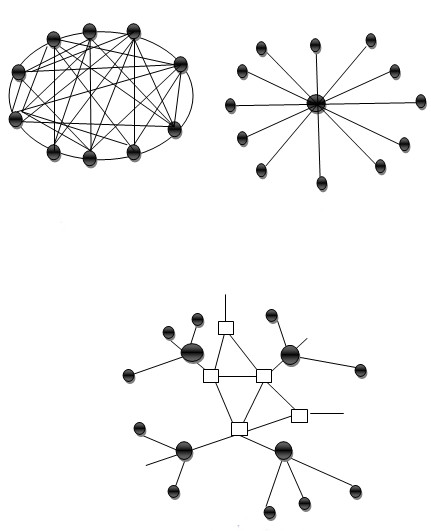
\includegraphics[width=30mm]{images/telephone_network.jpg}
\caption{(a) una rete completamente interconnessa, (b) commutatore centralizzato, (c) gerarchia a due livelli}
\end{figure}

\subsubsection{Modem, ADSL, Wireless}

Per inviare segnali digitali attraverso una linea telefonica, il computer deve convertire i dati in forma analogica; solo in questo modo le informazioni possono essere trasmesse attraverso un collegamento locale.
Il modem ha la funzione di convertire i dati dalla forma digitale del pc alla forma analogica. Nella centrale poi i dati vengono ritrasformati in digitale e poi ritrasmessi in linee a lunga distanza. Dall'altro capo poi ci sarà il modem per la conversione inversa alla precedente. 
I problemi principali delle linee di trasmissioni sono 3:

\begin{enumerate}

\item{\textbf{Attenuazione}: rappresenta la perdita di energia (in dB/Km) causata dalla propagazione del segnale verso l'esterno. Tale perdita dipende dalla frequenza};
\item{\textbf{Distorsione}: rappresenta la differenza di velocità all'interno del cavo tra le varie componenti del segnale};
\item{\textbf{Rumore}: rappresenta l'energia indesiderata all'interno del segnale originale, causate da sorgenti di trasmissione esterne}.

\end{enumerate}

\begin{figure}[htbp]
\centering
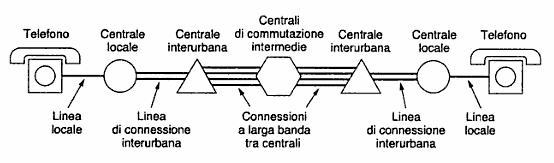
\includegraphics[scale=1]{images/phone.png}
\caption{Percorso tipico di una chiamata a media distanza}
\end{figure}

\subsubsection*{Modem}

Per riuscire a inviare dati in forma digitale è necessario un ampio spettro di frequenza questo rende adatta la trasmissione in banda base (DC) solo a basse velocità e distanze brevi. Il problema è aggirato utilizzando una trasmissione (\textbf{AC}) aggiungendo un segnale portante tra i 1000 e i 2000 Hz. Nella \textbf{modulazione di ampiezza} (ASK) sono utilizzate 2 diverse ampiezze 0 e 1, nella \textbf{modulazione di frequenza} (FSK) si utilizzano 2 o più toni. Nella forma più semplice di \textbf{modulazione di fase}, l'onda portante è spostata sistematicamente di 0 oppure 180 gradi a intervalli uniformi.

\begin{figure}[htbp]
\centering
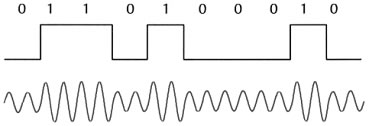
\includegraphics[scale=1]{images/modulazione_ask.jpg}
\caption{Modulazione d'ampiezza}
\end{figure}

\begin{figure}[htbp]
\centering
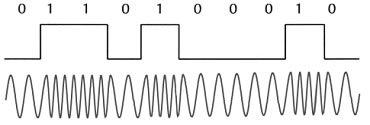
\includegraphics[scale=1]{images/modulazione_fsk.jpg}
\caption{Modulazione di frequenza}
\end{figure}

\begin{figure}[htbp]
\centering
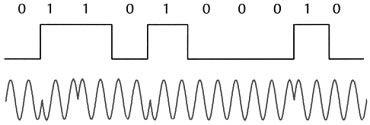
\includegraphics[scale=1]{images/modulazione_psk.jpg}
\caption{Modulazione di fase}
\end{figure}

Un apparecchio che utilizza uno di questi metodi per ``tradurre'' un flusso di bit in segnale analogico è detto \textbf{modem}. La maggior parte dei modem campiona 2400 volte al secondo. Il numero di campionamenti al secondo si misura in \textbf{baud}. Durante ogni baud è trasmesso un simbolo.
Concetti da ricordare:

\begin{itemize}
\item{\textbf{Banda passante}: intervallo di frequenza passante nel mezzo con un attenuazione minima, varia da 0 a una frequenza massima e si misura in Hertz};
\item{\textbf{Baud rate}: numero di campioni per secondo (=frequenza simboli)};
\item{\textbf{Modulazione}: è una tecnica che determina il numero di bit per simbolo};
\item{\textbf{Frequenza di bit}: quantità di $(simboli/sec)*(bit/simbolo)$}.

\end{itemize}

Tutti i modem evoluti utilizzano una combinazione di tecniche di modulazione per trasmettere più bit per baud. Spesso per trasmettere diversi bit/simbolo si combinano insieme più ampiezze e spostamenti di fase.

La trasmissione digitale è adatta in banda base (DC) a basse velocità. Per aggirare i problemi di tale banda si usa la trasmissione AC introducendo un segnale costante detto \textbf{portante d'onda sinusoidale}. La sua ampiezza, frequenza o fase posso essere modulate per inviare informazioni. Nella \textbf{modulazioni di ampiezza} vengono usate 2 ampiezze diverse per rappresentare 1 e 0 mentre in quella di \textbf{frequenza} (FSK) si utilizzano più toni. Infine nella \textbf{modulazione di fase} più semplice l'onda viene spostata di 0 o 180 gradi (schemi migliori utilizzano spostamenti più piccoli). I modem odierni utilizzano modulazioni ibride per avere un maggior baud rate. Un esempio è la QPSK (\textit{Quadrate Phase Shift Keying}). Questa tecnica di modulazione prevede l'utilizzo di più fasi e più ampiezze, e in base al numero di combinazioni nascono i nomi QAM-16 (4 bit per simbolo utilizzando 4 fasi e 4 ampiezze, 9600 bps), QAM-64 (\textit{Quadrature Amplitude Modulation})e così via.

\begin{figure}[htbp]
\centering
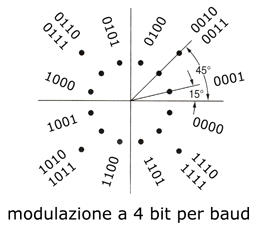
\includegraphics[scale=1]{images/qam.png}
\caption{Diagramma costellazione QAM}
\end{figure}

Uno schema con costellazione molto fitta è soggetto a errori, per questo i modem che li adottano utilizzano meccanismi di correzione degli errori, per esempio con un bit extra di parità.
Gli standard utilizzati dai modem più conosciuti sono:

\begin{itemize}

\item{\textbf{V.32}: trasmette 4 bit più 1 di parità a 2400 baud (9600 bps)};
\item{\textbf{V.32 bis}: trasmette 6 bit più 1 di parità a 2400 baud (14400 bps)};
\item{\textbf{V.34}: utilizza 12 bit per simbolo a 2400 baud (28800 bps)};
\item{\textbf{V.34 bis}: utilizza 14 bit per simbolo a 2400 baud (33600 bps)}.

\end{itemize}

Una connessione che permette ai dati di viaggiare in entrambe i sensi è detta \textbf{full duplex}; un esempio di linea full duplex è una strada a due corsie. Una connessione che permette ai dati di scorrere in entrambi i sensi ma ha solo un senso alla volta è chiamata \textbf{half duplex}; un esempio di linea half duplex è il binario ferroviario. Infine, una connessione che permette di trasmettere i dati in una sola direzione è chiamata \textbf{simplex}; un esempio di linea simplex è una strada a senso unico. 
In base a quanto detto la velocità massima dei modem è 34 Kbps; questo non è vero perché l'ampiezza del canale telefonico è 4 MHz, quindi per Nyquist il numero di campioni massimo è 8000, per gli 8 bit per campione usato negli U.S. si hanno 64 Kbps. In realtà non è così, perché 1 bit serve per il controllo, per cui si riduce il tutto a 56 Kbps, che è lo standrard \textbf{V.90}. Lo standard successivo al V.90 si chiama \textbf{V.92}. I modem che adottano questo standard possono raggiungere una velocità di trasmissione di 48 kbps, se la linea è in grado di gestirla.

\subsubsection*{Linee DSL}

I servizi con un'ampiezza di banda superiore a quella del servizio telefonico standard si dicono \textbf{a banda larga}; il termine, comunque, rappresenta più un concetto di merketing che un concetto tecnico.
Inizialmente ci furono molte offerte sovrapposte, tutte raccolte sotto un unico nome: \textbf{xDSL}.
I modem sono così lenti perchè i telefono sono stati inventati per trasmettere la voce umana e l'intero sistema è stato attentamente ottimizzato per questo scopo. Nel punto in cui ogni collegamento locale termina nella centrale locale, il cavo attraversa un filtro che attenua tutte le frequenze sotto i 300 Hz e sopra i 3400 Hz. Il limite non è netto, perciò l'ampiezza di banda si considera solitamente 4000 Hz. I dati sono perciò limitati a questa stretta banda.
Il trucco che fa funzionare xDSL è che quando un cliente si abbona a questo servizio, la linea di ingresso viene collegata a un diverso tipo di commutatore che, non usando questo filtro, rende disponibile l'intera capacità del collegamento locale.
I servizi xDSL sono stati progettati tenendo conto di alcuni obiettivi:

\begin{enumerate}

\item I servizi devono funzionare sui doppini di categoria 3 esistenti adoperati per i collegamenti locali;
\item Non devono influire sugli apparecchi telefonici e sui fax in dotazione degli utenti;
\item Devono essere molto più veloci della connessione a 56 kbps;
\item Dovrebbero essere sempre attivi e avere un costo mensile non legato al tempo di utilizzo.

\end{enumerate}

Il primo servizio \textbf{ADSL}, offerto da AT\&T, divideva lo spettro disponibile sui collegamenti locali in tre bande di frequenza: \textbf{POTS} (\textit{Plain Old Telephone Service}), \textbf{upstream} (dall'utente alla centrale) e \textbf{downstream} (dalla centrale all'utente). La tecnica basata su diverse bande di frequenza è chiamata \textbf{multiplexing} a divisione di frequenza.
Le offerte successive proposte da altri fornitori hanno seguito un approccio diverso, che poi si è dimostrato vincente. L'approccio alternativo, chiamato \textbf{DMT} (\textit{Discrete MultiTone}) divideva lo spettro in 256 canali indipendenti. Il fornitore del servizio decide quanti canali utilizzare per la trasmissione e quanti per la ricezione. Una combinazione 50 e 50 è tecnicamente possibile, ma la maggior parte dei fornitori assegna al canale utilizzato per scaricare i dati l'80-90\% dell'ampiezza di banda, poichè la maggior parte degli utenti preleva più di quanto trasmetta. Questa soluzione fa nascere la ``A'' (Asimmetrica) di ADSL. Di solito 32 canali sono dedicati alla trasmissione e il resto alla ricezione.
Dentro ogni canale si utilizza uno schema di modulazione simile a quello di V.34, dove la velocità di campionamento è di 4000 baud invece di 2000. La qualità della linea è tenuta strettamente sotto controllo e la velocità dati è regolata continuamente, perciò canali differenti possono avere velocità diverse.
Il model ADSL è in realtà un elaboratore di segnali digitali, che fa le veci di 250 modem QAM che operano in parallelo a diverse frequenze. Poichè la maggior parte dei modem ADSL è esterna, il computer deve essere collegato all'apparecchio attraverso una connessione veloce; di solito si utilizza una scheda Ethernet oppure una porta USB.

\begin{figure}[htbp]
\centering
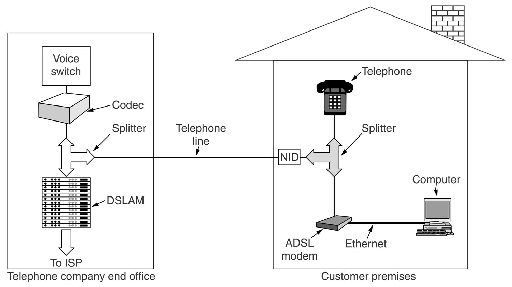
\includegraphics[width=120mm]{images/adsl_configuration.png}
\caption{Una tipica configurazione ADSL}
\end{figure}


\subsubsection{Multiplexing}

Per limitare i costi le aziende hanno ideato modi per convogliare più conversazioni nello stesso mezzo fisico, appunto il\textbf{ Multiplexing}. Esistono sostanzialmente 2 categorie di quest'ultimi:

\begin{itemize}

\item{FDM: Frequency Division Multiplexing};
\item{TDM: Time Division Multiplexing};

\end{itemize}

In FDM lo spettro fi frequenze è diviso in bande e ogni utente ne possiede una. In TDM gli utenti si danno il cambio, tipo round-robin.

\subsubsection*{Multiplexing a divisione di frequenza}

La banda è limitata dai filtri a 3.1 KHz, e nell'unione in multiplexing viene allocato uno spazio un po superiore, 4 KHz per avere un po di tolleranza. Poi ogni canale voce viene aumentato di una frequenza diversa e unito agli altri senza sovrapposizione. Nonostante questi accorgimenti 2 canali adiacenti avranno u po di sovrapposizione che potrebbe tramutarsi in un po di rumore nei 2 canali. Uno standard comune prevede 12 canali voce uniti in multiplexing nella banda tra 60-108 KHz. Questa unità è chiamata \textbf{gruppo} che possono essere uniti in multiplexing in un \textbf{supergruppo} e a loro volta ancora in un \textbf{mastergroup}.

\subsubsection*{Multiplexing a divisione di lunghezza d'onda}

Utilizzato per i canali in fibra, il \textbf{WDM} (\textit{Wavelenght Division Multiplexing}) si fonda sul principio della combinazione e divisione di lunghezze d'onda. Più fibre vengono combinate convogliando ogni segnale in un unico canale nella cui estremità c'è uno splitter utile a ripristinare i segnali delle fibre di partenza. La differenza sostanziale rispetto all'FDM è il sistema ottico completamente passivo. Un sistema con molti canali e lunghezze d'onda ravvicinate è definito \textbf{DWDM} (Dense WDM).

\subsubsection*{Multiplexing a divisione di tempo}

Gestita completamente da dispositivi elettronici digitali, per cui è necessaria una conversione da parte della centrale prima di trasmettere il segnale sulla linea di uscita. La centrale locale digitalizza il segnale analogico producendo numero a 8 bit (grazie al \textbf{codec}, \textit{coder-decoder}), elaborano  8000 campioni al secondo. Questa tecnica è chiamata PCM e costituisce il cuore del sistema telefonico odierno. Nel mondo esistono molti schemi PCM diversi incompatibili tra loro. In Giappone e in Nord America si utilizza la portante T1 in altre zone del mondo quella E1. Una tecnica chiamata \textbf{differential pulse code modulation} al posto di inviare l'ampiezza digitalizzata invia la differenza rispetto alla precedente così da ridurre il numero di bit (da 7 a 5) utili supponendo che sia poco probabile il salto di \(\pm\)16. Una variante di questa tecnica detta \textbf{modulazione delta} si basa su un principio simile: ogni valore campionato differisce dal precedente di \(\pm\)1 sotto le condizioni che può essere trasmesso un singolo bit che dice se il nuovo campione è maggiore o minore del precedente. Questa tecnica che ipotizza una bassa variazione di segnale può avere problemi con bruschi cambiamenti di livello. Esistono altre tecniche dette \textbf{codifiche per ipotesi} che utilizzando pochi valori precedenti prevedono il successivo.

\subsubsection{Commutazione}

\subsubsection*{Commutazione di circuito}

Quando viene avviata una telefonata l'apparecchio di commutazione del sistema telefonico prova a creare un percorso fisico tra il chiamante e il chiamato. 

\subsubsection*{Commutazione di messaggio}

Questa tecnica non prevede un collegamento fisico a priori ma si basa su un idea diversa, ovvero un passo alla volta. Il messaggio viene inviata alla prima centrale di commutazione, la quale dopo averlo esaminato per vedere gli eventuali errori, lo ritrasmette alla successiva fino ad arrivare al destinatario. Questa tecnica è chiamta di \textbf{store and forward}.

\subsubsection*{Commutazione di pacchetto}

Questa tecnica è molto diversa dalle precedenti e si basa sull'idea di dividere i dati in pacchetti limitati i quali partono e possono arrivare anche in ordine sparso sarà compito del destinatario riordinarli. Non c'è bisogno di alcun collegamento predefinito e ogni pacchetto può percorrere strade diverse. E' più resistente agli errori della commutazioni di circuito , poiché si possono aggirare commutatori bloccati passando per un altro percorso. Inoltre la commutazione di pacchetto non riserva alcuna ampiezza di banda per cui in linea generale è più efficiente. L'addebito dipende sia dal tempo che dalla distanza.

\begin{figure}[htbp]
\centering
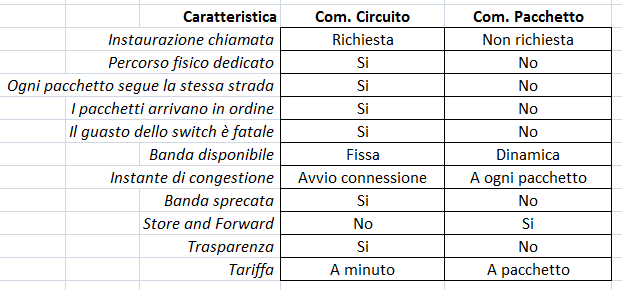
\includegraphics[scale=0.8]{images/comm.png}
\caption{Confronto tra commutazioni}
\end{figure}

\subsection{Sistema telefonico mobile}

Esistono 3 generazioni di telefoni cellulari:

\begin{enumerate}

\item{Voce analogica};
\item{Voce digitale};
\item{Voce e dati digitali}.

\end{enumerate}

\subsubsection{Cellulari di I generazione}

Il primo esempio di ``cellulare'' lo si ha nel 1946 quando venne creato il sistema premi e parla, come ad esempio quella dei CB. Negli anni sessanta scompare il tasto per parlare grazie all' IMTS (\textit{Improved Mobile Telephone System}) che utilizzava un trasmettitore ad alta potenza posto in una collina, il quale utilizzava 2 frequenze, una per la ricezione e una per trasmettere. IMTS utilizzava solo 23 canali distribuiti tra 150 e 450 MHz. Il numero limitato di canali faceva si che alcuni utenti dovevano aspettare molto prima di aver segnale libero.

\subsubsection*{Sistema telefonico mobile avanzato}

Cambiò tutto grazie a AMPS (\textit{Advanced MPS}). Ogni area geografica era divisa in \textbf{celle}, in AMPS grandi 10-20 Km. Ogni cella utilizzava un insieme di frequenze diversa da quelle vicine. L'utilizzo di celle piccole richiede meno potenza. L'idea principale sta proprio qui, in celle piccole e grande riutilizzo delle frequenze. Nelle aree in cui il numero di utenti è elevato e il sistema tende a sovraccaricarsi ,le celle vengono a loro volta divise in \textbf{microcelle} così da aumentare il riuso delle frequenze. Tanto più piccole sono le celle tanto meno potenti devono essere i dispositivi. Da notare il fatto che una frequenza utilizzata da una cella non è più usata nell'area cuscinetto attorno ad essa (area di circa 2 celle). Al centro di ogni cella si trova una stazione la quale è collegata a un dispositivo chiamato MTSO (\textit{Mobile Telephone Switching Office}) o MSC(Mobile Switching Center). In sistemi più grandi sono necessari più MTSO che quindi vengono divisi in livelli. Ogni MTSO colloquia con gli altri. Un telefonino in ogni istante è logicamente posizionato in una certa cella e ogni qualvolta il segnale in tale cella si affievolisce, la stazione base colloquia con le adiacenti per delegare la gestione dell'apparecchio alla cella col segnale più forte. Questo processo è chiamato \textbf{handoff} e richiede 30 msec. Esistono 2 tipi di handoff:

\begin{itemize}

\item{soft handoff: l'acquisizione della nuova stazione avviene prima di interrompere il segnale precedente};
\item{hard handoff: la vecchia stazione rilascia il telefono prima che la nuova lo acquisisca. La chiamata viene bruscamente interrota}.

\end{itemize}

\subsubsection*{Gestione della chiamata}

Ogni telefono AMPS ha un numero seriale di 32 bit e un numero di telefono 10 cifre. Ogni volta che viene acceso, il telefono esplora i vari canali e trova il segnale più potente. Il telefono quindi trasmette in broadcast il proprio seriale e il numero di telefono con un codice di correzione degli errori. La stazione base aggiorna l' MTSO e ogni 15 minuti circa aggiorna la posizione corrente. Per chiamare il telefono acceso invia il numero del chiamato e i propri dati attraverso il canale di accesso e quando riceve la richiesta la stazione base informa l'MTSO. Se il chiamante appartiene a quell'MTSO cerca un canale libero per la chiamata, e trasmette il numero del canale al telefono. Il processo di ricezione è diverso: ogni telefono è in ascolto nel canale di trasferimento e quanto l'MTSO riceve il pacchetto che richiede il destinatario lo passa alla stazione base la quale chiede conferma al telefono. In caso affermativo la stazione invia il numero del canale con la chiamata e inizia la conversazione.

\subsubsection{Cellulari di II generazione}

Nel mondo sono sostanzialmente utilizzati  4 sistemi: D-AMPS, GSM, CDMA e PDC utilizzato solo in Giappone e molto simile al D-AMPS.

\subsubsection*{D-AMPS (\textit{Digital} AMPS)}

Il D-AMPS è totalmente digitale. Progettato per coesistere con AMPS utilizza gli stessi canali a 30 KHz con le stesse frequenze. Si è resa disponibile una nuova banda di frequenza 1850-1910 MHz per sostenere l'aumento del carico. Alcuni cellulari erano in gradodi utilizzare entrambe le bande disponibili. Su un telefono D-AMPS il segnale voce preso dal microfono viene digitalizzato e compresso dal \textbf{vocoder}, questa compressione permette la condivisione di una coppia di frequenze (upstream/downstream) fino a 3 utenti con multiplexing a divisione di tempo. Ogni coppia di frequenza supporta 25 frame/sec di 40 msec. Ogni frame è diviso in 6 slot temporali. Gruppi di 16 frame costituiscono un superframe, con alcune informazioni di controllo. Concettualmente funziona come AMPS: viene acceso il telefono, viene contattata la stazione e poi rimane in ascolto.
Nei tempi in cui il cellulare non riceve ne trasmette viene testata la qualità della linea. Questa tecnica è chiamata \textbf{MAHO}(\textit{Mobile Assisted HandOff})

\subsubsection*{Comunicazioni GSM \textit{(Global System for Mobile communications)}}

Molto simile ad D-AMPS però ha i canali più ampi così possono supportare ben 8 utenti in una coppia di frequenze. Un sistema GSM ha 124 coppie di canali simplex ampi 200 KHz e supporta 8 connessioni grazie a multiplexing a divisione di tempo. A ogni stazione attiva è assegnato uno slot temporale su una coppia di frequenze. Quindi teoricamente supporta 992 canali molti di questi però utilizzati come canali di controllo. Trasmissione e ricezione non avvengono nello stesso intervallo di tempo perché il sistema non è in grado di gestirlo. Questo protocollo ha introdotto le schede SIM che contengono al loro interno IMSI (identifica la SIM) e la chiave di crittografi (Ki). L'identificazione avviene così:

\begin{enumerate}

\item{Il cellulare manda Ki e IMSI in broadcast};
\item{L'operatore lo riceve e manda un numero casuale};
\item{Il cell lo rimanda firmato con Ki};
\item{L'operatore controlla}.

\end{enumerate}

Il \textbf{canale di controllo broadcast} è un flusso continuo di dati trasmessi dalla stazione base che annuncia identità e stato del canale. Il \textbf{canale di controllo dedicato} è utilizzato per aggiornare la posizione, registrare il terminale nella rete e configurare la chiamata. Infine c'è un \textbf{canale di controllo comune} che è diviso in 3 sottocanali logici. Il primo è il \textbf{canale di paging} utilizzato dalla stazione per annunciare le chiamate in arrivo. Poi c'è il \textbf{canale ad accesso casuale} e permette agli utenti d richiedere uno slot sul canale di controllo dedicato. Infine c'è il \textbf{canale di assegnazione dell'accesso} che assegna il lo slot del canale di controllo dedicato per ripetere le richieste efettuate dal secondo canale.

\subsubsection*{CDMA \textit{(Code Division Multiple Access)}}

Miglior sistema rispetto a quelli presentati e base per la III generazione a volte chiamato \textbf{cdmaOne}. CDMA permette la trasmissione per tutto il tempo attraverso l'intero spettro. Queste trasmissioni multiple simultanee vengono separate tramite tecnica di codifica. L'idea sta nel fatto che i segnali si sommino linearmente. Per cui tutti comunicano ma ogni coppia lo fa in ``lingua diversa''. Per risalire a ciò che viene detto basta togliere il rumore aggiunto dalle conversazioni di altri. Per riuscire a filtrare tale segnale rumoroso vengono utilizzate le matrice di Hadamard. Tecnicamente il CDMA funziona così:\\ ogni tempo di bit è diviso in m intervalli chiamati \textbf{chip} (generalmente 64-128 chip per bit) e ad ogni stazione viene assegnata una \textbf{sequenza di chip} univoca. Per trasmettere un 1 la stazione deve semplicemente inviare tale sequenza se invece invia uno zero deve farne il complemento. Non sono ammessi altri schemi. Per aumentare la quantità di informazione inviabile basta passare da b bit/sec a mb chip/sec aumentando l'ampiezza di banda di un fattore m. CDMA è una forma di comunicazione a spettro distribuito. Ognuna di queste sequenze di chip sono mutualmente ortogonali, ovvero ogni prodotto interno normalizzato di qualunque coppia di sequenze è uguale a 0 (ottenute con i \textbf{codici Walsh}). 
\[ S*T = \frac{1}{m}\sum\limits_{i=1}^m S_i T_i = 0\]
Da cui si deduce che S*S = 1 e S*\(\overline{S}\) = -1. 
Ora, ogni stazione invia queste sequenze come bit le quali si ``mischiano'' con le altre, tecnicamente si sommano con gli altri segnali di altre stazioni. Una volta che il segnale arriva alla stazione di destinazione per sapere il bit inviato dalla sorgente basterà moltiplicare il segnale per la sequenza di chip della sorgente e si otterrà il bit inviato.
Matematicamente se si deve capire il messaggio C allora sarebbe \textbf{S = A + \(\overline{B}\) + C}:
\[S*C = (A+ \bar{B} + C)*C = A*C + \bar{B}*C + C*C = 0 + 0 + 1 = 1\]
Per la proprietà di ortogonalità tutti i prodotti si sono annullati a parte quello interessato. Questo sistema è in genere utilizzato per reti wireless.

\subsubsection{Cellulari di III generazione}

La prima proposta di cellulari di III generazione fu fatta dall'ITU con l'intenzione di lanciarli nell'anno 2000 con ampiezza di banda di 2 MHz e 2Mbps per tutti. Un sogno irrealizzabile che ha visto il tutto slittare qualche anno più avanti e con alcune specifiche smussate come i 2Mbps per chi stava fermo e circa 400 per gli utenti che camminavano e 144 per quelli che si spostano a più alte velocità. I servizi che avrebe dovuto fornire IMT-2000 (così si chiamva la proposta) erano:

\begin{itemize}

\item trasmissione voce ad alta qualità;
\item trasmissione messaggi;
\item applicazioni multimediali;
\item accesso internet.

\end{itemize}

Per riuscire ad utilizzare questi servizi in tutto il mondo si era pensati di creare un unica tecnologia per rendere tutto più semplice. Furono fatte diverse proposte.

\subsubsection*{W-CDMA (\textit{Wideband CDMA})}

Questo protocollo fu proposto da Ericsson. In Europa battezzato col nome \textbf{UMTS} \textit{(Universal Mobile Telecommunications System)}. Si basa sui fondamenti del CDMA utlizzando però una banda larga a 5 MHz ed è stato progettato per interagire con il sistema GSM anche se non compatibile. Data rate 384 Kbps.

\subsubsection*{CDMA2000}

Proposto da Qualcomm, simile al precedente con la differenza di non interagire con GSM. Altre differenze col precedente sono il tempo di frame, di spettro e una diversa tecnica di sincronizzazione. Data rate 144 Kbps.

\subsubsection*{EDGE \textit{(Enhanced Data for GMS Evolution)}}

Uguale al GSM con un numero maggiore di bit per baud che comportano però più errori per baud. Sistema pensato durante il passaggio da II a III generazione, definito infatti 2.5G.

\subsubsection*{GPRS \textit{General Packet Radio Service}}

Altro schema per 2.5G. Una rete di pacchetti costruita sopra ad D-AMPS e GSM. GPRS permette di inviare e ricevere pacchetti IP in una cella basata su sistema vocale. Quando attivo alcuni slot temporali vengono dedicati al traffico dei pacchetti. Questi slot sono divisi in canali logici. Ogni canale è utilizzato per scaricare i pacchetti nei quali c'è indicato il destinatario. Per inviare un pacchetto la stazione mobile richiede uno o più slot e effettua la richiesta alla base. La base poi invia il pacchetto via internet tramite rete via cavo.

\subsubsection{Oltre al 3G}

\subsubsection*{HSDPA \textit{(High Speed Downlink Packet Access)}}

\subsubsection*{HSUPA \textit{(High Speed Uplink Packet Access)}}

\subsubsection*{HSOPA \textit{(High Speed OFDM Packet Access)}}

\newpage
\clearpage
\section{Lo strato data link}

\subsection{Progetto dello strato data link}
Lo strato data link si prende carico di diverse funzioni, fra cui:

\begin{enumerate}

\item{Definire un servizio di interfaccia per lo strato network};
\item{Gestire gli errori di trasmissione};
\item{Regolare il flusso di dati in modo che i dispositivi riceventi lenti non vengano sopraffatti dai trasmettitori veloci}.

\end{enumerate}

Per raggiungere questi obiettivi, lo strato prende i pacchetti che arrivano dallo strato network e li incapsula in \textbf{frame}, con uno \textit{header}, un \textit{corpo} e una \textit{coda}.

\begin{figure}[htbp]
\centering
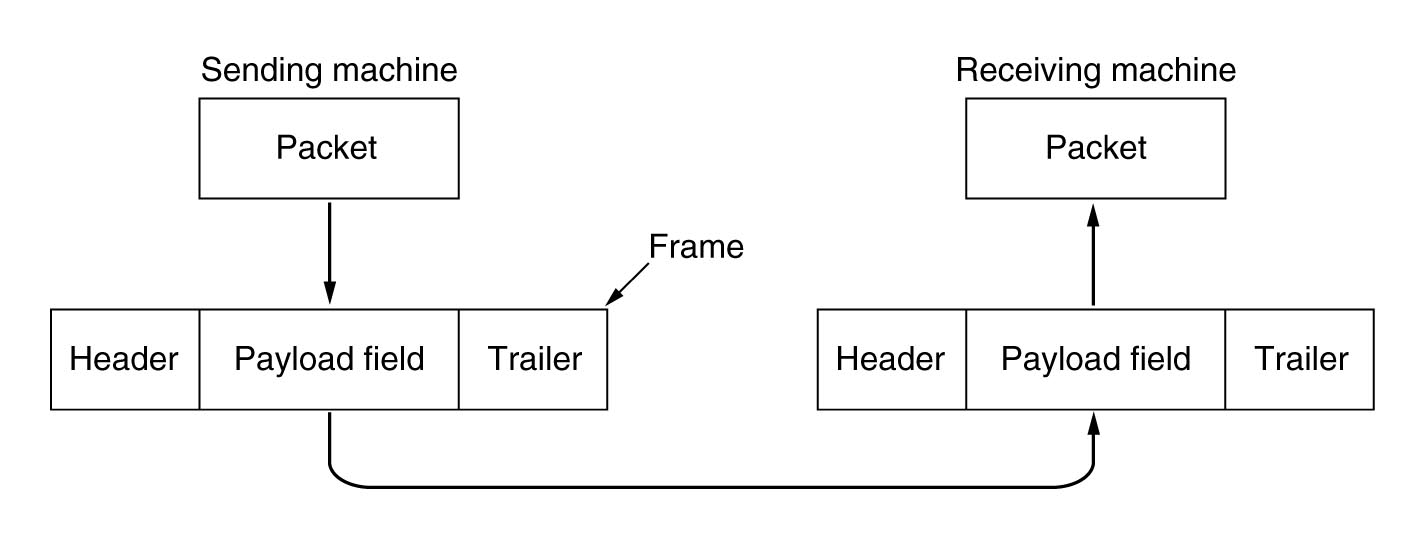
\includegraphics[scale=1]{images/package_frame.jpg}
\caption{Relazione fra pacchetti e frame}
\end{figure}

\subsubsection{Servizi}

La funzione dello strato data link consiste nel fornire servizi allo strato network. Il servizio principale è quello di trasferire dati dallo strato network della macchina sorgente allo strato network della macchina destinazione. Tre servizi che vengono comunemente forniti a questo livello sono:

\begin{enumerate}

\item{\textbf{Servizio unacknoledged senza connessione}: una macchina invia dei frame e non è necessaria una connessione dedicata e nemmeno una risposta e/o conferma del destinatario. Se il pacchetto viene perso non viene fatto nulla. Utile per canali con bassa percentuale di errori o per trasmissioni voce in cui il ritardo è peggiore di un errore};
\item{\textbf{Servizio acknoledged senza connessione}: anche qui non è necessaria una connessione, ma ogni frame è inviato singolarmente e si attende una conferma, entro un limite di tempo massimo, del destinatario. Se il limite è superato si reinvia il frame. Servizio utile per reti poco affidabili come le reti wireless};
\item{\textbf{Servizio acknoledged orientato alla connessione}: c'è bisogno di connessione tra le parti, poi si inizia a inviare. Ogni frame viene numerato. Tramite ACK viene garantita la ricezione e grazie alla numerazione si cerca di rilevarli nell'ordine esatto. Alla fine la comunicazione viene chiusa liberando i relativi buffer, variabili e risorse usate per mantenere la connessione}.

\end{enumerate}

\subsubsection{Suddivisione in frame}

Per servire lo strato network, lo strato data link deve usare a sua volta il servizio che gli è fornito dallo strato fisico, che ha come compito quello di prendere un flusso di bit e cercare di portarli a destinazione.
Il tipico approccio di questo strato consiste nel suddividere del flusso di bit in frame e calcolarne il cheksum, il quale viene ricalcolato dal destinatario che controlla la corrispondenza. In caso contrario si è verificato un errore e vengono presi i provvedimenti necessari. Un problema non banale è capire la suddivisione in frame, ovvero dove finisce o inizia un frame. Esistono 4 modi principali per farlo:

\begin{enumerate}

\item{Conteggio dei caratteri}
\item{Flag byte con byte stuffing}
\item{Flag di inizio e fine con bit stuffing}

\end{enumerate}

Il \textbf{primo metodo} banalmente inserisce nella testa un campo con il numero di caratteri di lunghezza del frame. Il problema principale è l'errore nel conteggio di caratteri durante la trasmissione che sfaserebbe tutto. Richiedere la ritrasmissione non è una soluzione perché il destinatario non capisce quanti caratteri deve saltare. Il \textbf{secondo metodo} aggira il problema inserendo un byte prima e dopo ogni frame, chiamato \textbf{flag byte}. Quindi in caso di perdita di sincronizzazione basterà cercare questo byte speciale. Un possibile problema è che all'interno dei dati ci sia un flag byte. Per risolverlo basta che la sorgente in tali casi inserisca un \textbf{byte di escape} (\textit{ESC}) subito prima di ogni occorrenza e la destinazione provvederà a toglierli (\textbf{destuffing}). Questa tecnica è chiamata \textbf{byte stuffing} (o \textbf{character stuffing}). Paradossalmente un ESC deve essere preceduto a sua volta da un ESC! Il problema di questo metodo è il legame con la decodifica dei caratteri con 8 bit che non è sempre vera. Il \textbf{terzo metodo} applica una tecnica simile alla precedente: ogni frame comincia e finisce con un gruppo speciale di bit, 01111110, in sostanza un flag byte. Ogni volta che lo strato Data link della sorgente incontra cinque 1 inserisce uno 0 subito dopo. Questa tecnica è detta \textbf{bit stuffing}. Il destinatario ovviamente incontrando cinque 1 e uno 0 non deve far altro che eliminare lo 0 per ottenere il messaggio originale.

\subsubsection{Controllo degli errori}
Per riuscire a rilevare banalmente errori nella trasmissione dei dati principalmente le cose da fare sono:\\ogni frame deve avere un numero di sequenza in modo che la destinazione accetta solo i frame che non ha già ricevuto, la sorgente ha un timer utile per quando attende che l'ACK ritorni dal destinatario in modo da non fare attesa infinita. Se non riceve ACK in un tempo limite stabilito dal protocollo il messaggio viene reinviato.

\subsubsection{Controllo del flusso}
Esistono principalmente 2 tecniche per la gestione del flusso (evitando così sovraccaricamenti del desinatario):
\begin{enumerate}
\item{Tramite Feedback: la destinazione manda alla sorgente informazioni per darle il permesso di inviare altri dati o comunque per informarla dello stato in cui si trova.}
\item{Tramite limitazione di velocità: il protocollo contiene al suo interno un meccanismo che limita la velocità della sorgente senza utilizzo di feedback.}
\end{enumerate}

\subsection{Rilevazione e correzione degli errori}
\subsubsection{Codici per la correzione degli errori}
Esistono principalmente 2 tipi di decodifica: a semplice rilevazione di errori e a correzione di errore. Entrambe consistono nell'aggiunta di informazioni ridondanti per rilevare e nel secondo caso correggere gli errori. Le 2 tecniche vanno applicate ovviamente in ambiti differenti, la prima più indicata per trasmissioni veloci tipo con fibra, mentre la seconda per trasmissioni più rumorose come quelle wireless. \\
Come avviene l'identificazione di un errore: in primo luogo indichiamo con n la lunghezza di una \textbf{codeword} formata da m bit per il frame e r per il controllo (n = m+r). Confrontando ora 2 codeword di lunghezza uguale facendo semplicemente lo XOR troviamo tutti 0 se le parole coincidono oppure alcuni 1. La quantità di 1 presenti corrisponde alla \textbf{distanza di Hamming}. Una distanza di Hamming \textit{d} rappresenta il numero di errori per convertire una sequenza nell'altra. Essendo che non tutte le possibili \(2^m\) codeword sono accettabili, un modo per intuire la codeword esatta è enumerare tutte le possibili codeword e scegliere quelle con distanza di Hamming minima. In base a alla distanza d+1 della codifica si riescono a trovare d errori. Mentre per correggerne d ci vorrebbe una codifica con distanza 2d + 1. Un esempio lo è il bit di parità.

\subsubsection*{Codifica di Hamming}
Vengono inseriti nella sequenza di bit da inviare bit di parità posti nelle posizioni che sono una potenza di 2. Questi bit di parità sono legati ad alcuni bit di dati con la seguente regola: il bit di dati k-esimo è controllato da quei bit la cui somma forma k. Per esempio k = 11 = 1 + 2 + 8, allora il primo, secondo e ottavo bit sono quelli di parità per k. Quindi se troviamo errori di inversione nei bit 1,2 e 8 allora l'11 è invertito. Questa codifica corregge solo errori singoli. Esiste un trucco nell'invio di dati per correggere gli errori improvvisi, detti \textbf{burst}, che è quello di inviare le varie codeword sotto forma matriciale inviando i dati colonna per colonna in modo che gli errori burst siano solamente singoli bit per ogni riga e si sa che tramite hamming si possono correggere.

\subsubsection{Codifiche a rilevazione d'errore}
\subsubsection*{CRC \textit{(Cyclic Redundance Check)}}
L'idea di base è quella di trattare le sequenze di bit come coefficiente di polinomi. Si applica per cui l'aritmetica dei polinomi in modulo 2. Quindi addizioni e sottrazioni sono fatte con lo XOR. Un divisore sta in un dividendo se ha gli stessi bit. Quando si utilizza CRC la sorgente e la destinazione devono accordarsi su un \textbf{polinomio generatore} \textit{G(x)} che deve avere come primo e ultimo bit 1. Il frame da controllare, che corrisponde al polinomio \textit{M(x)}, deve essere di ordine maggiorne di G(x). L'idea è quella di aggiungere un checksum alla fine del frame in modo che il polinomio rappresentato dal frame col checksum sia divisibile per G(x). Per cui la destinazione riceve il polinomio e prova a dividerlo per G(x). Se c'è resto allora c'è errore.\\
Il calcolo del checksum avviene così:
\begin{enumerate}
\item{Posto r il grado di G(x), aggiungere r zeri alla fine del frame, così da avere m+r bit e corrisponde al polinomio \( x^r M(x)\)}
\item{Dividere la sequenza corrispondente a \( x^r M(x)\) per quella di G(x) usando la divisione modulo 2.}
\item{Sottrarre il resto, al massimo r bit, dalla sequenza corrispondente \( x^r M(x)\), sottrazione in modulo 2. Il risultato sarà \textit{T(x)}}
\end{enumerate}

\subsection{Protocolli Data Link elementari}
\subsubsection{Protocollo stop-and-wait}
Protocollo molto semplice per il controllo del flusso e si può utilizzare in canali simplex o half duplex. Quando il mittente invia un blocco aspetta che il ricevente invii una conferma (ACK). Lo svantaggio è l'attesa della risposta, ma in compenso non c'è bisogno di regolare la velocità. Gli errori possibili ora sono 2:
\begin{enumerate}
\item{Sul frame: ovvero non arriva mai a destinazione e quindi il mittente aspetta all'infinito. C'è bisogno di un timeout come detto precedentemente.}
\item{Sul ACK: la conferma non arriva al mittente, il quale al termine del time out reinvia il pacchetto. Al destinatario arriva 2 volte ma grazie al numero di pacchetto (vedi su) il pacchetto non viene preso in considerazione.}
\end{enumerate}
\subsection{Protocolli sliding window}
Un protocollo per il controllo di flusso sicuramente più efficiente di quello appena presentato. Un dettaglio sicuramente a suo favore è l'utilizzo della tecnica di \textbf{piggybacking}, che consiste nello sfruttare un messaggio del destinatario al mittente come 'passaggio' per il messaggio di conferma ACK, in modo da non perdere tempo e sfruttare maggiormente il canale di comunicazione. Il campo \textit{ack} è posto nella testa del frame. Sorge il problema di quando fare piggybacking, un attesa troppo lunga può rendere vano il tutto perché il mittente fa un reinvio del frame. Quindi se il pacchetto arriva velocemente viene fatto piggybacking dell'ACK altrimenti si invia l'ACK separatamente. L'essenza del protocollo è che ogni partecipante alla comunicazione deve tener sotto controllo 2 finestre: quella dei frame in entrata e quella dei frame in uscita. Ogni frame in uscita contiene un numero di sequenza e il destinatario deve tener traccia di questi per la ricezione mentre il mittente per l'invio. 
\begin{figure}[htbp]
\centering
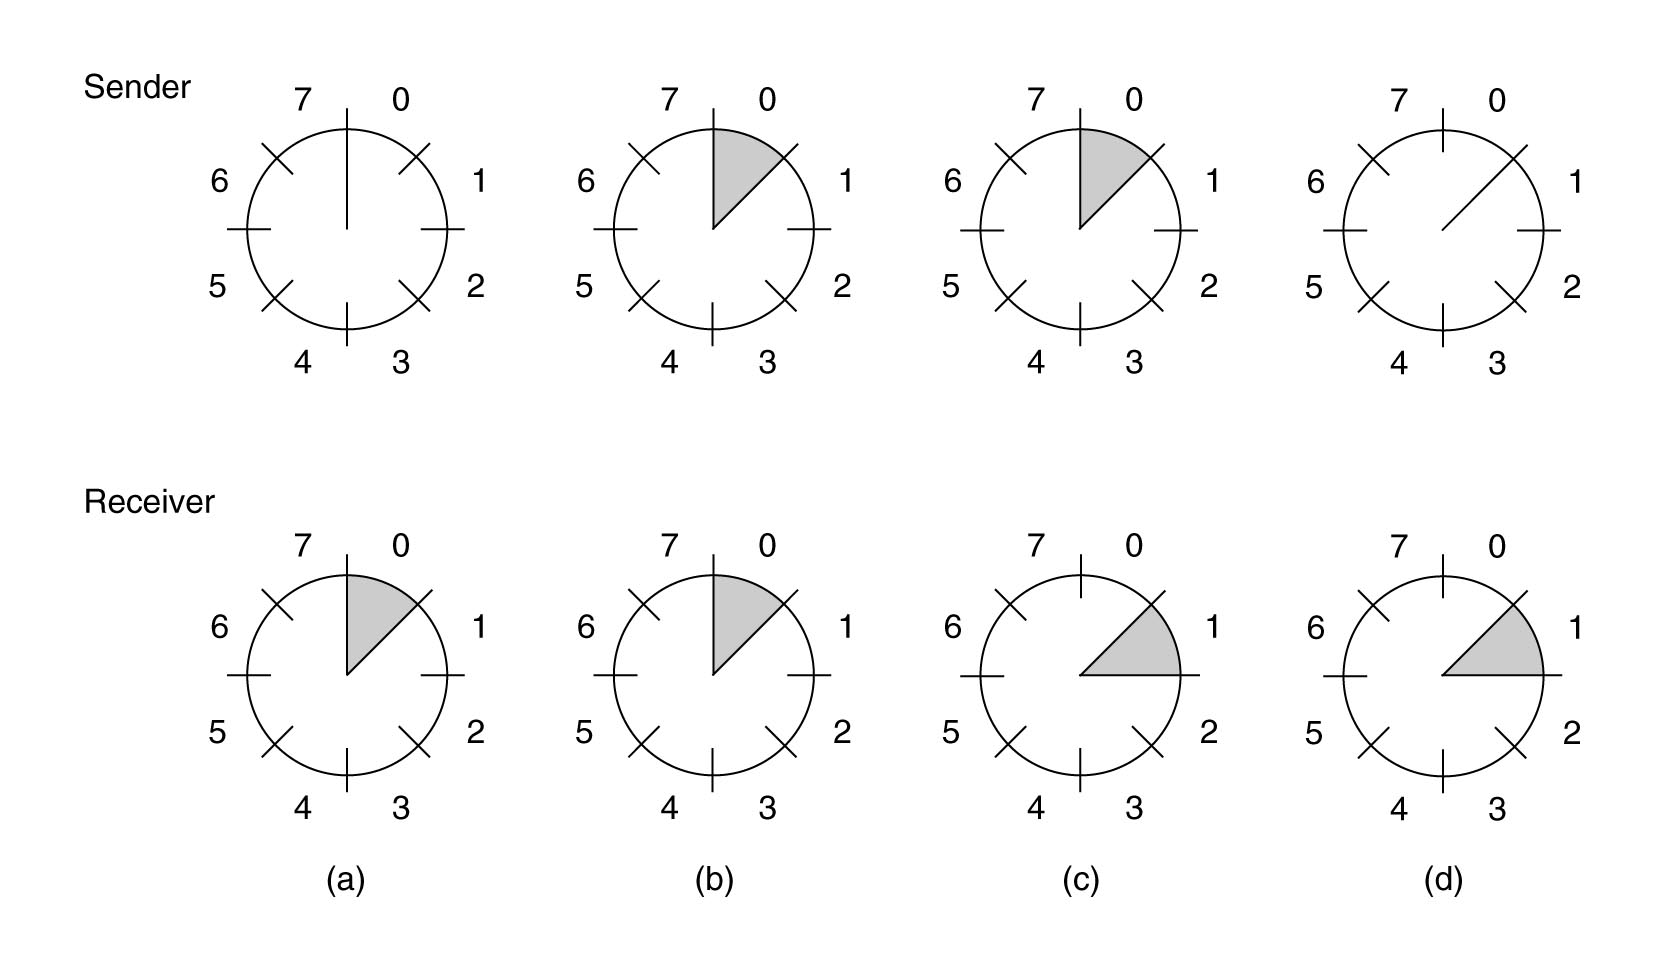
\includegraphics[scale=0.7]{images/sw.jpg}
\caption{Esempio sliding window: (a) Inizialmente, (b) Dopo l'invio del frame 0, (c) Dopo la sua ricezione, (d) Dopo l'invio dell'ACK.}
\end{figure}

\subsubsection{Protocollo sliding window a 1 bit}
La finestra di controllo ha dimensione 1 e viene utilizzato il metodo stp-and-wait. Quando il mittente invia un frame resta nella finestra finché non viene ricevuto l'ACK corrispondente prima di aggiornare la finestra. I frame inviati sono numerati con 1 o 0. Quando il destinatario riceve il frame controlla che il numero sia uguale a quello che aspettava, se si invia l'ACK. Se l'ACK contiene il numero che la sorgente si aspettava allora continua a inviare un nuovo pacchetto altrimenti reinvia quello segnato nel buffer. Si può utilizzare anche la tecnica \textbf{pipelining}, ovvero vengono inviati più frame contemporaneamente prima di entrare in attesa. Il destinatario aggiorna la finestra non appena riceve il frame e invia l'ACK. Esistono 2 approcci per contro i problemi di trasmissione durante il pipelining: uno chiamato \textbf{go back n} che semplicemente scarta tutti i frame dopo quello danneggiato, l'altra è la \textbf{ripetizione selettiva} nel quale vengono tenuti i frame buoni e non scartati e vengono messi in un buffer. Quando la sorgente va in timeout solo quello senza ACK viene rispedito. La destinazione quando trova un errore non sta "ferma", ma invia un NAK in modo da stimolare la ritrasmissione prima del timeout.

\subsubsection{Protocollo che usa go back n}
Qui la finestra di invio ha dimensione \(>\) 1 mentre quella di ricezione è uguale a 1. I pacchetti arrivano uno alla volta e su di essi viene fatto il checksum, se si trovano errori vengono segnalati alla sorgente indicando il numero del pacchetto danneggiato, per questo la finestra sorgente deve essere capiente. Se la finestra sorgente si riempie prima che il timer scatti, la pipeline viene svuotata. Le conferme vengono sempre mandate in piggybacking. La destinazione nel frattempo scarta i pacchetti successivi a quello avente l'errore. Questo approccio può far perdere molta banda se la frequenza degli errori è alta.
\begin{figure}[htbp]
\centering
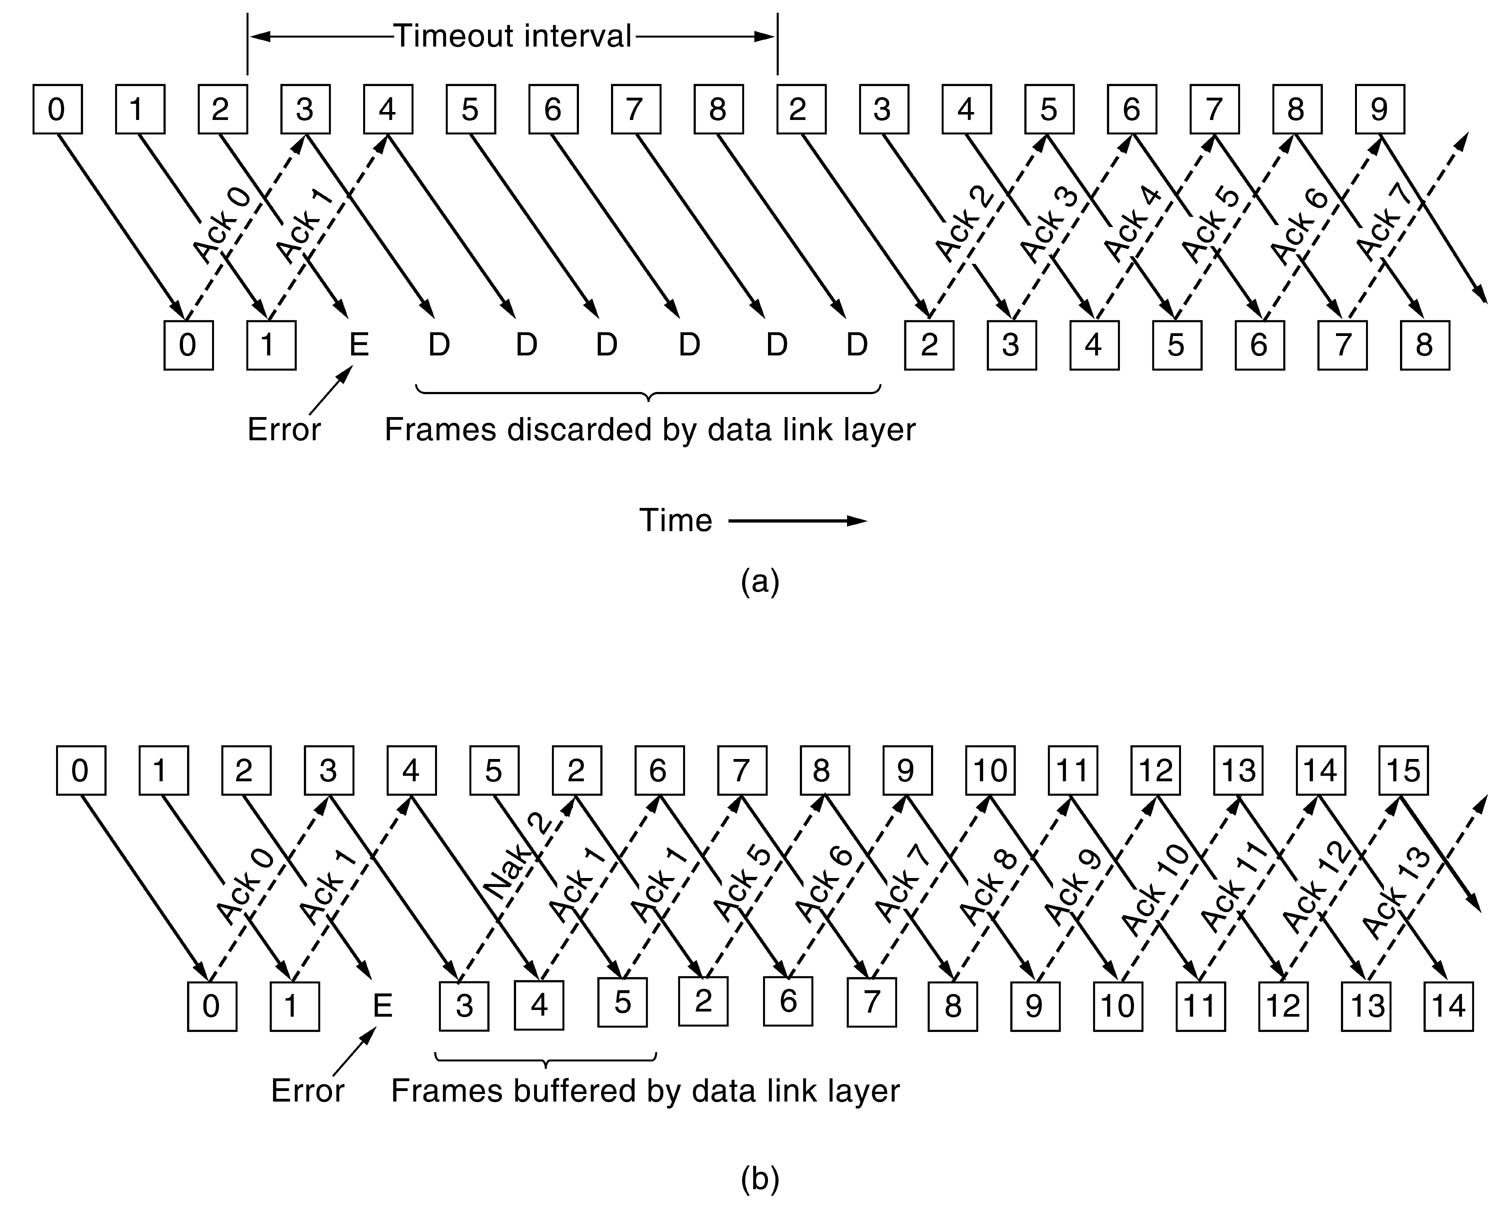
\includegraphics[scale=0.7]{images/gobackn.jpg}
\caption{Esempio sliding window con \textit{go back n}: effetti del pipelining.}
\end{figure}

\subsubsection{Protocollo che usa ripetizione selettiva \textit{(selective repeat)}}
In questo caso il buffer della destinazione deve essere più capiente. Nel caso di errori viene inviato alla sorgente un NACK (\textit{Not ACK}) indicandone il pacchetto. Finché il pacchetto errato non arriva nuovamente dalla sorgente i pacchetti successivi vengono posti nel buffer. Una volta arrivato tutto viene passato allo strato Network. \textit{Nota}: la sorgente dispone di timer per cui se non arrivasse il NACK il pacchetto viene reinviato comunque.

\subsection{Protocolli data link}
\subsubsection{HDLC (High-level Data Link Control)}
Deriva dal protocollo SDLC della IBM con le varianti LAP e LAPB. E' un protocollo orientato ai bit e usa il bit stuffing. La struttura dei frame di questo protocollo è:
\begin{figure}[htbp]
\centering
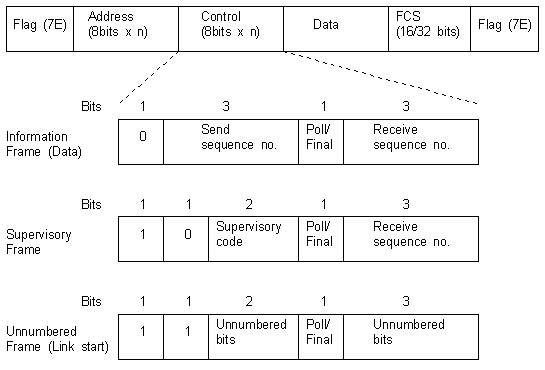
\includegraphics[scale=0.8]{images/hdlc.png}
\caption{Struttura frame HDLC}
\end{figure}
FCS indica la parte di checksum eseguita con CRC, Flag(7E) è il flag 01111110, mentre il Control con le Sliding Window e determina 3 tipi di frame:
\begin{enumerate}
\item{\textbf{Information}: formato da uno 0 seguito dal numero del frame. Poi p/f è utile per le conversazioni multiple e infine ci sono gli ACK (piggybacking sul frame successivo).}
\item{\textbf{Supervisory}: formato da uno 10 seguito dal campo type che può assumere 4 valori:
\begin{enumerate}
\item {Type 0: Frame ACK (Receive Ready)}
\item {Type 1: Frame NACK (Reject)}
\item {Type 2: Canale congestionato (Receive NOT Ready)}
\item {Type 3: NACK selettivo (Selected Reject)}
\end{enumerate}
Il resto come il precedente.}
\item{\textbf{Unnumbered}: formato da uno 11. Viene usato nel caso di perdita di frame.}
\end{enumerate}

I principalei comandi sono:
\begin{itemize}
\item{DISC: blocca la connessione}
\item{SNRM: nuova macchina on-line}
\item{SAMB: crea una connessione bilanciata}
\item{FRMR: rifiuta un frame di controllo}
\end{itemize}

\subsubsection{PPP \textit{(Point-to-Point Protocol)}}
Usato nei collegamenti punto a punto tra router e utente, ovvero in internet. Tra le varie funzioni di PPP troviamo: rilevazione degli errori, supporto per più protocolli, possibilità di negoziazione IP, possibilità di effettuare autenticazione. Tra le caratteristiche di questo protocollo meritano menzione:
\begin{enumerate}
\item{Metodo di framing che permettere di limitare i vari frame in modo non ambiguo e il formato del frame permette la rilevazione degli errori}
\item{Protoccolo di collegamento per gestire la connessione, i test, le negoziazioni e la gestione pulita della disconnessione. (LCP)}
\item{Modalità per negoziare le opzioni relative allo strato Network.}
\end{enumerate}
Utilizza 2 protocolli speciali:
\begin{enumerate}
\item{\textbf{LCP}\textit{(Link Control Protocol)}: insieme di comandi per la gestione del flusso e della comunicazione}
\item{\textbf{NCP}\textit{(Network Control Protocol)}: si occupa del dialogo con lo strato 3}
\end{enumerate}
La differenza più importante dall'HDLC è l'utilizo del byte stuffing.
Il frame PPP è così composto:
\begin{figure}[htbp]
\centering
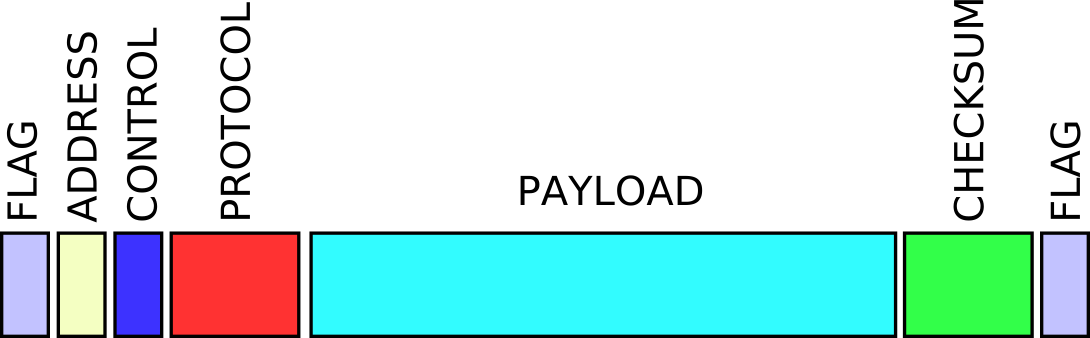
\includegraphics[scale=0.3]{images/ppp.png}
\caption{Struttura frame PPP}
\end{figure}
\begin{itemize}
\item{\textbf{FLAG}: flag byte tipico 01111110}
\item{\textbf{Address}: non viene usato, tutti 1}
\item{\textbf{Control}: posto per default a 00000011, ovvero niente controllo}
\item{\textbf{Protocol}: segnala il tipo di pacchetto che si invia}
\item{\textbf{Payload}: campo dati}
\item{\textbf{Checksum}: usa CRC}
\item{\textbf{FLAG}: di nuovo flag byte tipico}
\end{itemize}
\clearpage
\section{Il sottostrato MAC (\textit{Medium Access Control})}
\clearpage
\section{Capitolo Strato Network}
\clearpage
\section{Capitolo Strato Trasporto}
\clearpage
\section{Capitolo Strato Applicazione}
\clearpage
\section{Capitolo Sicurezza}

\appendix

\section{Glossario}

\section{Domande degli appelli}

\subsection{Capitolo 2}

\subsubsection{Cosa si intende per serie di Fourier}

Le informazioni possono essere trasmesse via cavo variando alcune proprietà fisiche, come la
tensione e corrente. Fourier condusse alcuni studi ed arrivò alla conclusione che le informazioni
trasmesse via cavo potevano essere rappresentate da una funzione $f(t)$. Questa funzione è
composta da una serie infinita di somme di seni e coseni, ed è in grado di rappresentare un segnale
periodico e regolare. La trasmissione però non è mai perfetta e c'è per forza attenuazione di linea.
L'intervallo di frequenze trasmesse senza forte attenuazione è detto \textbf{banda passante}.
Anche in un ipotetico canale perfetto, ovvero senza attenuazioni, la velocità di trasmissione non
può essere troppo elevata; la massima velocità è data dall'equazione di Nyquist/Shannon:

\begin{center}

$V_{max} = \log_{2} V  bit/sec$

\end{center}

\subsubsection{Bitrate e baudrate}

Bitrate: Velocità di trasmissione si indica in $bit/s$. Il teorema di Nyquist mette in relazione il bitrate con la banda disponibile:

\begin{center}

	$2H\log_2V$

\end{center}

Con H banda disponibile e V livelli di segnale (simboli) usati:

\begin{center}

	$S/N = segnale/rumore$,  $SNR = 10\log_{10} (S/N) dB$
	\newline
	$Massimo bitrate = 2\log_2 (1+(S/N))$

\end{center}	

Baudrate: numero di imboli al secondo, un simbolo può valere più bit.


\subsubsection{Descrivere i vari tipi di cavo e confrontarli}

Principalmente esistono 3 tipi di cavo, il classico \textbf{doppino}, il \textbf{cavo coassiale} e la \textbf{fibra}.

Il doppino è composto da due conduttori di rame isolati, attorcigliati tra loro in modo
elicoidale (DNA style), per evitare interferenze fra di loro. Il doppino è molto utile per la linea
telefonica, dato che può percorrere molti km senza che il segnale si indebolisca, ovvero senza
bisogno di un'amplificazione.

Il cavo coassiale è più grosso e può estendersi per distanze maggiori rispetto il doppino. La distanza
maggiore è frutto di una maggior schermatura a cui è sottoposto il nucleo in rame del cavo che lo
rende immune dal rumore. Esistono due cavi coassiali, uno da 50 Ohm per le trasmissioni digitali e
uno da 75 Ohm per quelle analogiche.

La fibra ottica è formata da 3 parti: sorgente luminosa, mezzo di trasmissione e rilevatore di luce. La
sorgente di luce è rappresentata da LED oppure laser, anche se il secondo, oltre ad essere meno
diffuso è anche più costoso. Il mezzo trasmissivo è la fibra, composta un nucleo di vetro di pochi
micron, avvolta in una guaina di vetro rivestita a sua volta da una guaina di plastica. La luce che
attraversa la fibra è riflessa al suo interno, da un'estremità all'altra del cavo. Nonostante si
trasmetta alla velocità della luce, quest’ultima viene stroncata dalla velocità di decodifica inferiore
che avviene alle estremità. La fibra può contenere più raggi che si differenziano per l'angolo di riflessione. Questo tipo di fibra è detto multimodale. Se la trasmissione all'interno della fibra è
unica, si ha una trasmissione in linea retta, detta monomodale.

Lo svantaggio della fibra rispetto al doppino e cavo coassiale è il costo maggiore e la difficoltà
nell'unire vari pezzi di cavo, mentre per gli altri due tipi basta attorcigliare il nucleo di rame. Il
vantaggio della fibra è la manutenzione, essendo vetro è pari a zero. Altro vantaggio è l'unione di
più canali, che avviene tramite prismi.

\subsubsection{Caratteristiche e confronto fra i vari tipi di satellite, GEO, MEO, LEO}

Un satellite è un grande ripetitore di microonde posizionato in cielo. Ci sono tre tipi di satelliti che si
differenziano per la loro distanza dalla superficie terrestre.

I satelliti più lontani sono detti \textbf{geostazionari} e sono posti in successione su un’orbita circolare al livello dell’equatore, ad una distanza minima di 2 gradi uno dall'altro( ps: immaginare tanti cerchi
concentrici che hanno come primo cerchio il nostro equatore e tutti gli altri più grandi, i satelliti
sono su uno di questi). Questi satelliti sono molto lontani dalla terra e per questo hanno un tempo
medio di ritardo della trasmissione di 300 millisecondi, ma con uno di essi possiamo coprire quasi
un terzo della superficie terrestre. I satelliti \textbf{LEO} distano circa 500 km dalla terra, hanno un tempo di latenza inferiore rispetto ai GEO, come il consumo energetico. Essendo vicini, per coprire tutta la
terra, sono necessari molti satelliti. Si muovono velocemente. I satelliti \textbf{MEO} sono posti a un'orbita intermedia tra i LEO e GEO, hanno una velocità relativamente bassa, in quanto sono posti a 18 mila
km dalla terra e il loro tempo di rivoluzione è di 6 ore.

\subsubsection{Che cos'è la modulazione in frequenza (FM)? E in ampiezza(AM)?}

La modulazione in frequenza è una delle tecniche di trasmissione utilizzate per inviare informazioni
attraverso la variazione della frequenza dell’onda portante. La FM è una modulazione a onda
continua, ovvero viene modulata la portante sinusoidale.
Per riuscire a inviare dati in forma digitale è necessario un ampio spettro di frequenza, questo
rende adatta la trasmissione in banda base solo a basse velocità e a distanze brevi. Nella
modulazione a frequenza vengono utilizzate 2 o più frequenze.

\textbf{Pro}:

\begin{itemize}

\item Molto meno sensibile ai disturbi rispetto all’AM;
\item Permette una trasmissione di miglior qualità;
\item Efficienza energetica molto maggiore, cioè il segnale di informazione non richiede potenza aggiuntiva per essere trasmesso.
\item 

\end{itemize}

\textbf{Contro}:

\begin{itemize}

\item Necessità di circuiti molto più complessi;
\item Occupa più banda;
\item 

\end{itemize}

Modulazione in ampiezza (AM): due diverse ampiezze sono usate per rappresentare 0 e 1. Utilizza
per il segnale un segnale a radio frequenza come portante. L’AM modifica il segnale in modo
proporzionale.

\textbf{Pro}:

\begin{itemize}

\item Semplice da mettere in pratica.

\end{itemize}

\textbf{Contro}:

\begin{itemize}

\item Molto sensibile a disturbi.

\end{itemize}

\subsubsection{Che cos'è la modulazione delta (delta modulation)?}

Questa tecnica è una differente tecnica di multiplexing (più conversazioni nello stesso mezzo fisico)
a divisione di tempo. Ogni valore campionato differisce dal precedente di +1 o -1 sotto le condizioni
che può essere trasmesso un singolo bit che dice se il nuovo campione è maggiore o minore del
precedente.

\subsubsection{Descrivere in dettaglio il GSM (Global System for Mobile connection)}

Il GSM è una tecnologia simile al D-AMPS, appartenente alla seconda generazione di cellullari con
qualche modifica. La prima sostanziale è il numero di canali, infatti il GSM ha 124 coppie di canali
simplex ampi 200KH e supporta fino ad 8 connessioni contemporanee grazie al multiplexing a
divisione di tempo. La trasmissione e la ricezione non avvengono nello stesso intervallo, poiché il
sistema non è in grado di gestirlo. Il GSM è il protocollo che ha introdotto le SIM, le quali
contengono IMSI e la chiave crittografia KI, diversa per ogni SIM. Il cellulare manda IMSI e KI in
broadcast. L'operatore riceve entrambi e invia un numero casuale, che viene analizzato e
rimandato con la firma del KI all'operatore.

La struttura a cella GSM: nel protocollo GSM ci sono 4 tipi di celle: macro, micro, pico e Umbrella.
Le prime sono le più grandi, sono sopraelevate rispetto gli edifici e hanno un raggio massimo di 35
km. Le micro sono più piccole, coprono un'altezza pari agli edifici. Le pico sono molto piccole, usate
in aree molto dense, tipicamente indoor. Umbrella è una piccola estensione, usata per coprire i
buchi tra le varie celle sopracitate.

\subsubsection{Si descriva la tecnica CDMA (Code Division Multiple Access), possibilmente con esempio}

CDMA permette la trasmissione per tutto il tempo attraverso l'intero spettro. Queste trasmissioni
multiple e simultanee vengono separate tramite tecnica di codifica. L'idea è che i segnali si
sommino linearmente, ma ogni coppia lo fa in lingua diversa. Per risalire a ciò che viene detto,
basta togliere il rumore aggiunto dalle altre conversazioni utilizzando le matrici di Walsh. Vediamo
un esempio.

Creando una matrice di Hadamard 4x4 posso gestire 4 lingue, invertendo ogni riga ottengo altre 4
parole, in modo da avere una coppia di parole per ogni lingua. Ognuno usa una parola, si sommano
le coordinate di ogni parola ottenendo un unico vettore risultante che moltiplicato per una parola
di una determinata lingua, fornisce un numero:

\begin{itemize}

\item \textbf{Zero}: se il dispositivo non ha trasmesso;
\item \textbf{Positivo}: c'è una parola in quella lingua e la parola è la parola positiva;
\item \textbf{Negativo}: c'è una parola in quella lingua e la parola è la parola negativa;

\end{itemize}

Es: Si costruisca una base trasmissiva (chip codes) per 18 stazioni in CDMA (volendo, usando le
matrici di Hadamard).
Basta fare la matrice di hadamard 32x32 e prendere solo 18 righe Il chip codes è una riga della
matrice (di Hadamard) che viene assegnata alla singola stazione che trasmette quello per mandare
un 1 o il complemento a 1 $(riga * -1)$ per mandare uno 0. Ogni riga definisce una ``lingua'' diversa che
è linearmente indipendente dalle altre (alias riga $S*T = S*(-1*T )= 0$ se $S != T$).

\subsubsection{Il GPRS: cos'è, difetti e pregi}

Il GPRS è un'evoluzione del GMS che permette la gestione del traffico a pacchetti. Al contrario del
GSM non serve un servizio dedicato ma vi è un canale condiviso. Lo spreco di banda è inesistente e
si utilizza una tariffa a traffico e non a tempo, come avviene per il GSM. IL GPRS aggiunge il
supporto a PPP e IP. essendo una naturale evoluzione del GSM, ci furono differenti classi di
cellulare, a seconda del supporto alla prima o seconda tecnologia.

Nei cellulari in classe C, l'utente deve selezionare quale comunicazione utilizzare, se GSM oppure
GPRS. La classe B, permette di utilizzare entrambe le reti, ma se si sta scaricando un pacchetto e si
riceve una chiamata, il download viene sospeso. Prima della classe A, esiste una pseudo classe A, in
cui si possono usare contemporaneamente utilizzando una solo frequenza. La Classe A, permette di
utilizzare sia una che l'altra tecnologia, contemporaneamente, è come avere due cellulari
indipendenti.

La sicurezza è analoga al GSM, con l’aggiunta di una seconda chiave Kc( cipher key). Questa è
generata ogni volta dalla Ki e da un numero casuale ogni volta che l’utente di autentica.

\subsubsection{Handoff: che cos’è e i vari tipi}

Nelle connessioni mobili, ogni telefono è connesso alla rete tramite una sola cella finché non si
sposta. Quando ci si sposta, si deve cambiare la cella precedente con una più vicina, anche per
evitare problemi dati dalla distanza. La disconnessione da una cella, può avvenire con due modalità:

\begin{itemize}

\item Hard handoff: quando il segnale è troppo debole, lo switching office chiede alle celle vicine
quanta potenza ricevono dal cellulare. Queste gli rispondono e il cellulare viene riassegnato
alla cella con più potenza. Quindi il cellulare viene mollato e poi riagganciato, in qualche
caso è presente del lag che fa cadere la linea;
\item Soft handoff: introdotto da GSM per ovviare al problema del lag, quando il cellulare ha
poco segnale dalla cella, prima di lasciarla, si aggancia ad una nuova e poi abbandona la
vecchia. Occorre che il cellulare gestisca due frequenze, cosa che 1G e 2G non supportavano.

\end{itemize}

\subsubsection{FDM, TDM, CDM: algoritmi per la selezione della banda}

FDM: sfrutta la trasmissione in banda passante per condividere un canale, divide lo spettro in
bande di frequenza di cui ogni utente ha uso esclusivo per inviare il proprio segnale.

TDM: gli utenti fanno a turni secondo una politica round-robin e ognuno di loro, periodicamente
prende possesso della banda completa per un tempo limitato.

CDM: comunicazione a spettro distribuito in cui un segnale a banda stretta viene sparso su una
banda di frequenza più ampia. Ciò rende il segnale più tollerante alle interferenze e permette a più
segnali di utenti diversi di condividere la stessa banda di frequenza, chiamato anche CDMA.

\subsubsection{QAM e QAM16 (Quadrature Amplitude Modulation)}

È un sistema di modulazione numerica sia analogica che digitale. Le portanti sono solitamente
sinusoidali. Il termine quadratura indica che gli angoli differiscono di $90 ^{\circ}$. Il segnale può essere visto
come la somma di due segnali modulati in fame.

QAM: Più immune al rumore si ottiene tramite i diagrammi a costellazione, quelli circolari sono
quelli ideali ma sono più difficili sia da ottenere che da decodificare.
QAM 16: Quando si voleva spingere sull’acceleratore, nella trasmissione di dati via cavo, si è
pensato che il miglior approccio da utilizzare era combinare due tipi di modulazione assieme,
l’ampiezza e la fase.

Da questa idea nasce il QAM-16. Grazie ad esso possiamo utilizzare un alfabeto più ampio e spedire
un simbolo su 16 ogni unità di tempo con bitrate quadruplo.
\section{Capitolo 3}

\subsubsection{Che cos'è il byte stuffing?}

Il byte stuffing è usato in PPP (Point-to-Point Protocol) ed è un metodo usato per capire dove inizia e finisce un frame. Il byte stuffing inserisce prima e dopo ogni frame un byte, chiamato flag byte.
Quindi in caso di perdita di dati, basterà cercare l'ultimo flag byte caricato. Un possibile
inconveniente è che dentro i dati ci sia un flag byte. In questo caso, basta che la sorgente inserisca un byte di Escape subito prima di ogni occorrenza e la destinazione provvederà a toglierli.
Il controllo del frame è eseguito dallo strato Data Link, il quale prima di passa passare il frame allo strato successivo, elimina le sequenze escape e i flag byte.

Se trova una sequenza di escape nel frame, devo inserire a sua volte un altro escape per non far
ignorare le successiva. Un difetto di questo metodo è legato all’uso di caratteri a 8 bit. Ad esempio Unicode usa una codifica a 16bit.

\subsubsection{Descrivere il Bit stuffing}

È analogo al byte stuffing, solo che è fatto a livello di bit, così viene aggirato il problema del byte stuffing e quindi si può scegliere la dimensione della flag. Ogni frame inizia e finisce con 01111110 (protocollo X.25). Ogni volta che lo strato datalink della sorgente incontra 5, uni di fila inseriscono uno zero. Il destinatario ogni volta che incontra 5 uni, elimina lo zero successivo. Questo metodo è usato anche per fare padding.

\subsubsection{Numero di bit necessari per riconoscimento(correzione) degli errori di trasmissione}

Esistono due strategie per la gestione degli errori:

\begin{itemize}

\item Codifica a correzione d’errore: vengono inclusi nel blocco trasmesso una quantità di
informazioni ridondanti, che in caso di errore permettono di ricostruire e riparare il frame;
\item Codifica a rilevazione di errori: introduce ridondanze in modo che il destinatario capisca se
c’è un errore, ma NON è in gradi di correggerlo.

\end{itemize}

Dati m bit per il frame e r bit ridondanti: $m+r=n$, ovvero n è la lunghezza totale del messaggio
inviato, chiamato codeword. Prendiamo ad esempio due codeword: 810001001 e 10110001. Come determino quanti bit corrispondenti sono differenti? Eseguo l’OR esclusivo ed ottengo 0011000. Il numero di bit corrispondenti diversi è detto distanza di Hamming: se due codeword sono a distanza di Hamming d uno dall’altra, sono necessari d errori su singoli bit per convertire una sequenza nell’altra. Per trovare d errori necessito di codifica con distanza d+1. 
Per correggere d errori necessito di codifica con distanza 2d+1.

\subsubsection{Si descriva cos'è il CRC (Cycle redundancy check). Si calcoli inoltre il CRC di 10011101 usando il polinomio generatore di $x^4+x+1$.}

Il cyclic redundancy check è un metodo per il calcolo di checksum. Il nome deriva dal fatto che i dati d'uscita sono ottenuti elaborando i dati di ingresso, i quali vengono fatti scorrere ciclicamente in una rete logica. Il controllo CRC è molto diffuso perché la sua implementazione binaria è semplice da realizzare, richiede conoscenze matematiche modeste per la stima degli errori e si presta bene a rilevare errori di trasmissione su linee affette da elevato rumore di fondo. 16) il generatore deve avere i bit di ordine più alto e più basso uguali a 1. per poter calcolare il checksum di un frame di m bit che corrisponde al polinomio M(x), il frame deve essere più lungo del polinomio generatore.

Quando la destinazione riceve un frame prova a dividerlo per il polinomio generatore. Se la
divisione ha un resto, c'è stato un errore nella trasmissione.

\begin{enumerate}

\item Posto r il grado di G(x), aggiungere r bit con valore zero dopo la parte di ordine piu'
basso del frame. Così che adesso contenga m+r bit e corrisponda al polinomio $x^r M(x)$;
\item Dividere la sequenza di bit corrispondenti a G(x) per la sequenza corrispondente a $x^r
M(x)$ usando la divisione modulo 2;
\item Sottrarre il resto dalla sequenza corrispondente a $x^r M(x)$ usando la sottrazione in
modulo 2. Il risultato è il frame con checksum pronto per la trasmissione.

\end{enumerate}

Dati due polinomi P e G (generatore) dobbiamo aggiungere alla destra di P tanti zeri quanto è il
grado massimo di G e otteniamo il polinomio F. Poi si dive il polinomio ottenuto per G, si ottiene un resto che va sommato al polinomio F, infine si raggruppano i bit in gruppetti di 4 e si codifica in esadecimale.

Esempio: $P=10011101$ e $G= x^4+x+1$, quindi abbiamo $G=10011$, $F= P=100111010000$ e il resto è $1111$.

Il polinomio finale è $1001 1101 1111$ in esadecimale è $9DF$.

\subsubsection{Descrivere Il protocollo stop and wait, pregi e difetti}

Il protocollo S\&W è un protocollo molto semplice per il controllo del flusso e si può utilizzare in
canali simplex o half-duplex. Quando il mittente invia un blocco aspetta che il ricevente invii una
conferma, un ACK (acknowledge). Lo svantaggio principale è l'attesa, ma in compenso non c'è
bisogno di regolare la velocità.

Possono sorgere due errori: il frame non arriva mai a destinazione e il mittente aspetta e rinvia
all'infinito: c'è bisogno di un tempo limite di rinvio. L'altro problema riguarda l'ACK: potrebbe non arrivare al mittente, il quale rinvia il pacchetto e al destinatario arriva più volte, ma per fortuna viene scartato, grazie al numero di messaggio.

\subsubsection{Cos’è il piggybacking}

La tecnica consiste nello sfruttare un messaggio del destinatario al mittente come passaggio per
l’ACK, in modo da non perdere tempo e sfruttare al meglio il canale di comunicazione(un messaggio
in meno da inviare). Il campo ACK è posto all’inizio del frame. Il problema principale è quando fare
piggybacking: in attesa molto lunga può essere vana, poiché il mittente rinvia il frame. Quindi se il pacchetto arriva per il mittente è caricato e inviato in tempo breve si fa piggybacking, altrimenti s’invia l’ACK separatamente.

\subsubsection{Si descriva la tecnica dello Sliding window}

È un protocollo per il controllo di flusso. Utilizza la tecnica del piggybacking. Invia pacchetti e
aspetta messaggio di conferma ACK. Sorge il problema di quando fare il piggybacking, un’attesa
troppo lunga può rendere vano il tutto perché il mittente fa un rinvio del frame. Quindi se il
pacchetto arriva velocemente viene fatto piggybacking sennò viene inviato separatamente.
L’essenza del protocollo è che ogni partecipante alla comunicazione deve tener sotto controllo 2
finestre, quella dei frame in entrata e quella dei frame in uscita. Ogni frame in usciata contiene un numero di sequenza e il destinatario deve tener traccia di questi per la ricezione mentre il mittente per l’invio.

Con lo sliding window a 1 bit, viene utilizzato il metodo stop and wait. Quando il mittente invia un
frame, resta nella finestra finché non viene ricevuto l’ACK corrispondente prima di aggiornare la
finestra. I frame inviati sono numerati con 1 o 0. Quando il destinatario riceve il frame, controlla
che il numero sia uguale a quello che aspettava, se s’invia l’ACK. Se l’ACK contiene il numero che la sorgente si aspettava allora continua a inviare, altrimenti re invia quello segnato nel buffer. Si può utilizzare anche il pipelining, inviando più frame contemporaneamente prima di entrare in attesa. Il destinatario aggiorna la finestra non appena riceve il frame e invia l’ACK. Esistono 2 approccio: go back n e selective repeat.

\subsubsection{Si descriva l'idea dei protocolli ``go back N'', indicandone pregi e difetti.}

Questo protocollo è utilizzato con sliding window di ampiezza 1 in ricezione e maggiore di uno in
invio. I pacchetti arrivano uno per volta e su di essi viene fatto un checksum, se si trovano errori
vengono segnalati alla sorgente indicando il numero del pacchetto danneggiato. Per questo motivo la finestra deve essere capiente. Se la finestra sorgente si riempie prima che il timer di arrivo scatti, la pipeline viene svuotata. La destinazione intanto scarta i pacchetti successivi a quello in errore.

Questo approccio è efficacie contro la prevenzione di errori, ma occupa molta banda se la frequenza di errori è alta.

\subsubsection{Si descriva cos'è la tecnica del selective repeat}

La tecnica del selective repeat è una tecnica che si usa con il protocollo sliding window. In questo caso il buffer della destinazione deve essere più capiente. Infatti in caso di errori, viene inviato alla sorgente un NACK, indicandone il pacchetto. Finché il pacchetto contenente l'errore non arriva al destinatario, i pacchetti successivi vengono mantenuti nel buffer. Una volta arrivato tutto, il messaggio viene passato allo strato network. Inoltre la sorgente dispone di un timer per cui, se il pacchetto è errato e non arrivasse un NACK il pacchetto sarebbe rinviato comunque.

\section{Capitolo 4}
\section{Capitolo 5}
\section{Capitolo 6}
\section{Capitolo 7}
\section{Capitolo 8}

\end{document}